% =========================================================================
% Official IOP Publishing Journal Article — iopjournal.cls (2025)  [v2.0]
% Target Journal: Bioinspiration & Biomimetics (IOPscience, Q1)
% Template Source: https://publishingsupport.iopscience.iop.org/questions/latex-template/
% Revision: P1-P7 improvements applied 2026-08-16
% =========================================================================

\documentclass{iopjournal}

\usepackage{amsmath}
\usepackage{amssymb}
\usepackage{booktabs}
\usepackage{url}
\usepackage{subcaption}
\usepackage{siunitx}

\usepackage{pifont}
\newcommand{\cmark}{\ding{51}}% เครื่องหมายถูก ✓
\newcommand{\xmark}{\ding{55}}% เครื่องหมายกากบาท ✗

\begin{document}

\articletype{Paper}

\title{A Dual Time-Scale Artificial Hormone Mechanism for Fault-Tolerant CPG-Based Snake Robot Locomotion: Neuro-Endocrine Diffusion, Hill Receptor Gating, and Dynamic Spinal Bypass}

\author{Potiwat Ngamkajornwiwat$^{1,*}$\orcid{0000-0003-4050-4951}}

\affil{$^1$Department of Robotics and Automation Engineering, Faculty of Engineering and Technology, Panyapiwat Institute of Management, Nonthaburi 11120, Thailand}

\affil{$^*$Author to whom any correspondence should be addressed.}

\email{potiwatnga@pim.ac.th}

\keywords{snake robot, artificial hormone mechanism, fault-tolerant locomotion, reaction-diffusion dynamics, Hill receptor kinetics}

% =========================================================================
% [P3] REVISED ABSTRACT: Narrative-first, parameter-light (≤250 words)
%      Answers: Why? Gap? What? Found? Means?
% =========================================================================
\begin{abstract}
Modular snake robots are uniquely suited for navigating confined, unstructured environments such as disaster rubble and subsea conduits, yet remain highly vulnerable to in-field actuator failures. When a joint locks or loses power, the serpentine traveling wave fractures, causing lateral drift or complete locomotor paralysis. Existing fault-tolerant methods either rely on centralized fault detection routines—which suffer from diagnosis latency—or local proportional feedback laws that lack multi-segment spatial coordination.

Inspired by biological neuro-endocrine volume transmission, in which hormones diffuse through vertebrate spinal tissue to reorganize locomotor circuits after injury, we propose a \textbf{Local-Global Artificial Hormone-Gated CPG (AHM-CPG)} framework. The core insight is that proprioceptive kinematic coherence deficits can trigger decentralized hormone secretion, which propagates spatially along the spine via a 1D reaction-diffusion network, is steeply thresholded by Hill receptor kinetics, and drives adaptive CPG amplitude modulation, dynamic multi-hop phase bypass, and curvature offset neutralization—all without explicit fault identification.

We validate the framework across 480 simulation episodes in PyBullet, comparing 6 controllers under 8 fault modes and 7 environmental stress conditions. The proposed AHM-CPG controller achieves a mean forward velocity of $\SI{0.173}{\metre\per\second}$ (speed recovery ratio $\eta_{\text{rec}} = 69.1\%$, 95\% CI: $[61.0\%, 77.2\%]$), significantly outperforming all baselines ($p < 0.001$, Cliff's $\delta > 0.35$). In locked mid-joint scenarios, recovery reaches $119.7\%$ of the pre-fault speed. These results demonstrate that dual time-scale neuro-endocrine modulation provides a robust, model-free paradigm for bio-inspired robotic resilience, with promising implications for physical deployment.
\end{abstract}

%-----------------------------------------------------------------------
\section{Introduction}
\label{sec:intro}
%-----------------------------------------------------------------------

Limbless biological organisms, including snakes, eels, and caecilians, exhibit remarkable adaptive locomotion across complex and unstructured terrains by generating continuous traveling body waves~\cite{dickinson2000,hirose1993}. In biological systems, rhythmic undulatory motion is generated and coordinated by decentralized spinal neural circuits known as Central Pattern Generators (CPGs)~\cite{grillner2006,guertin2013,marder2001}. Remarkably, when vertebrates sustain neuromuscular fatigue, trauma, or spinal cord lesions, systemic neuro-endocrine modulators (such as serotonin, dopamine, and octopamine) diffuse through interstitial fluid and hemolymph to reorganize spinal network connectivity and restore functional stepping~\cite{courtine2008,rossignol2011,bargmann2012,sillar2014,edgerton2004}. This volume transmission mechanism operates concurrently across two distinct temporal scales: rapid synaptic transmission ($<100\text{ ms}$) and slow hormonal diffusion and clearance (seconds to minutes), conferring biological locomotion with graceful degradation and robust homeostasis.

Inspired by these biological mechanisms, modular snake-like robots have emerged as versatile platforms for navigating confined, hazardous, and extreme environments, including disaster rubble, subsea pipelines, and planetary surfaces~\cite{transeth2009,liljeback2012,wright2012,crespi2008}. Nevertheless, the high degree of articulation renders physical snake robots particularly vulnerable to mechanical and electrical actuator lesions in the field~\cite{schmucker2022,elsayed2021,sartoretti2019}. When an actuator locks at an arbitrary non-zero angle or suffers complete loss of power, three critical failure modes manifest: first, the continuous traveling curvature wave $q(s, t)$ fractures into disconnected anterior and posterior segments; second, the anisotropic ground friction mechanism ($\mu_{\text{lat}} \gg \mu_{\text{fwd}}$) necessary for forward propulsion collapses into uncoordinated lateral slip; and third, asymmetric ground reaction moments induce severe heading drift, spiral spinning, or complete locomotor paralysis.

Overcoming these mechanical vulnerabilities poses two fundamental theoretical challenges at the intersection of biological cybernetics and distributed robotic control. First, from a sensing and neuromodulation perspective, it remains elusive how local proprioceptive movement deficits can be mapped into a coordinated multi-segment spatial compensatory response without triggering spurious remodeling during transient tracking perturbations. Second, from a topological and dynamical perspective, standard decentralized oscillator networks lack mechanisms to autonomously bridge severed phase pathways across inactive or frozen modules, resulting in irreversible traveling wave decoherence unless mediated by centralized fault detection and isolation (FDI) routines that inevitably introduce diagnostic latency and single-point vulnerability.

To address these challenges, in this study we introduce a \textbf{Local-Global Artificial Hormone-Gated Central Pattern Generator (AHM-CPG)} framework, drawing direct inspiration from the neuro-endocrine volume transmission mechanisms that orchestrate functional recovery in vertebrate spinal cord injury~\cite{courtine2008,rossignol2011,bargmann2012} and adaptive biorobotic locomotion principles~\cite{wang2026,manoonpong2007,manoonpong2013,ijspeert2008}. By integrating proprioceptive kinematic coherence sensing with a 1D spatial reaction-diffusion signaling network and nonlinearly cooperatively gated Hill receptor kinetics ($m=6.0$), the proposed architecture dynamically suppresses oscillatory tracking noise while autonomously establishing multi-hop bypass phase bridges and neutralizing directional curvature bias—achieving emergent, model-free resilience without explicit fault diagnosis or supervisory intervention.

The primary contributions of this paper are fourfold:
\begin{enumerate}
  \item \textbf{Dual Time-Scale Neuro-Endocrine Architecture and Analytical Boundedness}: We formulate a four-stage decentralized control hierarchy that couples proprioceptive kinematic coherence sensing, 1D reaction-diffusion hormone dynamics, and cooperative Hill receptor kinetics. We provide a formal mathematical proof (Proposition 1) guaranteeing the non-negativity and uniform boundedness of the hormone state space under continuous fault excitation.
  \item \textbf{Dynamic Multi-Hop Spinal Bypass with Phase-Locking Stability}: We establish an autonomous inter-modular phase coupling mechanism that constructs multi-hop bridging links across lesions, providing an analytical proof of exponential phase error convergence ($\tau_{\text{sync}} \approx 156\text{ ms}$) to preserve traveling wave continuity without centralized clock remapping.
  \item \textbf{Decentralized Curvature Offset Neutralization and Actuator Thermal Protection}: We introduce an active endocrine counter-bias mechanism that eliminates directional heading drift under asymmetric locked angles, while simultaneously attenuating damaged joint drive to reduce actuator Joule heating dissipation ($\mathcal{E}_{\text{thermal}}$) by $86.4\%$, preventing permanent motor burnout in hardware deployment.
  \item \textbf{Factorial Benchmark Evaluation and Biological Reciprocity}: We conduct a comprehensive 480-episode simulation benchmark across six controllers, eight fault modes, and seven environmental stress regimes with rigorous non-parametric statistics (Cliff's $\delta$, Holm-Bonferroni corrections), accompanied by a 210-episode five-module ablation study that provides computational support for the primacy of receptor cooperativity in biological volume transmission.
\end{enumerate}

The remainder of this paper is organized as follows: Section~\ref{sec:related} reviews related work in CPG control, fault-tolerant modular robotics, and artificial hormone systems. Section~\ref{sec:methods} details the mathematical modeling of the four-stage AHM-CPG pipeline and provides analytical stability proofs. Section~\ref{sec:setup} describes the simulation environment, benchmark controllers, and evaluation metrics. Section~\ref{sec:results} presents quantitative experimental results, statistical benchmarks, and generalization tests. Section~\ref{sec:discussion} analyzes the ablation study, biological insights, and failure modes. Finally, Section~\ref{sec:conclusion} concludes the paper with future research directions.

%-----------------------------------------------------------------------
%-----------------------------------------------------------------------
% [P1] Background and Related Work Section
%-----------------------------------------------------------------------
\section{Background and Related Work}
\label{sec:related}

\subsection{CPG-Based Locomotion Control: From Biology to Modular Robotics}
Rhythmic motor behavior in vertebrate and invertebrate animals is fundamentally orchestrated by Central Pattern Generators (CPGs)—decentralized spinal neural circuits capable of generating coordinated, multi-phase rhythmic motor commands in the absence of descending cortical inputs or rhythmic sensory feedback~\cite{grillner2006,marder2001,delcomyn1980}. In biological snakes and anguilliform swimmers, distributed spinal networks establish smooth rostral-to-caudal traveling waves that generate continuous ground reaction propulsion against anisotropic friction scutes~\cite{dickinson2000,hirose1993}.

Translating these biological principles to robotic systems, Ijspeert~\cite{ijspeert2008} established $SO(2)$ limit-cycle oscillator networks as a canonical foundation for bio-inspired locomotion. By coupling non-linear dynamical systems across adjacent joints, CPGs achieve intrinsic phase-locking, smooth frequency modulation, and natural entrainment with sensory feedback. Prominent robotic realizations include the amphibious snake robot Amphibot~\cite{crespi2008}, adaptive obstacle-negotiating controllers by Wu and Ma~\cite{wu2010}, modular walking machines by Manoonpong et al.~\cite{manoonpong2007,manoonpong2013}, and omnidirectional quadrupeds by Matos and Santos~\cite{matos2014}. However, a ubiquitous design assumption across all these foundational frameworks is \textit{actuator structural integrity}—the underlying neural networks presume that all motor units faithfully execute commanded phase trajectories. Consequently, when an actuator suffers mechanical jamming or electrical failure, the rigid coupling topology causes traveling wave fracture, inducing severe locomotor degradation.

\subsection{Fault-Tolerant Locomotion in Modular Robotics}
To mitigate hardware vulnerabilities in articulated machines, roboticists have pursued two primary methodological paradigms:
\begin{enumerate}
  \item \textit{Model-Based Fault Detection and Isolation (FDI)}: These methods utilize analytical observers, extended Kalman filters, or parameter estimation algorithms to diagnose joint anomalies~\cite{elsayed2021,tanaka2015}. While providing rigorous diagnostic identification, FDI pipelines are inherently centralized, computationally burdensome, and subject to diagnostic latency ($>1.5\text{ s}$ in multi-joint systems), during which uncompensated ground reaction moments often destabilize the robot before corrective action can take effect.
  \item \textit{Reactive Sensory Feedback and Gait Reconfiguration}: Model-free approaches adjust locomotion parameters directly from proprioceptive mismatches~\cite{sartoretti2019,righetti2008}. Schmucker et al.~\cite{schmucker2022} developed fault-tolerant gait libraries for snake robots by pre-computing offline gait adaptations across enumerated failure modes. Elsayed et al.~\cite{elsayed2021} proposed local shape-based amplitude scaling on adjacent healthy joints. However, purely local feedback rules lack spatial coordination across non-adjacent segments, while pre-computed transition libraries cannot scale to unmodeled, compound, or environmental stress variations.
\end{enumerate}

\subsection{Bio-Inspired Neuromodulation and Artificial Hormone Systems}
In biological nervous systems, functional recovery from trauma does not rely solely on direct synaptic rewiring; instead, it is heavily governed by \textit{neuro-endocrine volume transmission}~\cite{bargmann2012,sillar2014}. Following traumatic spinal cord injury in mammals, systemic and paracrine neuromodulators (such as serotonin, dopamine, and noradrenaline) diffuse slowly through the spinal interstitial fluid, binding to high-affinity receptors to alter synaptic excitability and facilitate the emergence of indirect propriospinal relay pathways that bypass the injury site~\cite{courtine2008,rossignol2011,courtine2009}.

In cybernetics and distributed computing, Brinkschulte et al.~\cite{brinkschulte2007} formalized Artificial Hormone Systems (AHS) for decentralized task allocation and organic self-healing. Hamann and W{\"o}rn~\cite{hamann2008} and Schmickl and Crailsheim~\cite{schmickl2011} successfully deployed hormone-inspired reaction-diffusion fields to coordinate swarm robotic behaviors and multi-agent synchronization. Despite these successes in computing and swarm swarming, the concept of dual time-scale endocrine modulation has never been formulated for continuous multi-link serial kinematic chains to resolve structural actuator lesions.

\subsection{Reaction-Diffusion Dynamics and Morphogenetic Signaling}
Turing's seminal theory of morphogenesis~\cite{turing1952} and Meinhardt's subsequent mathematical formulations~\cite{meinhardt1982} demonstrated that coupled reaction-diffusion partial differential equations (PDEs) can generate stable spatial concentration profiles from purely local interactions. Arena~\cite{arena2000} demonstrated that cellular neural networks driven by reaction-diffusion dynamics can produce emergent spatio-temporal locomotor waves. In this work, we adopt a 1D spatial reaction-diffusion signaling continuum along the robot's spinal axis, incorporating non-linear saturation decay to establish a stable, self-limiting chemical communication channel across articulated joints.

\subsection{Critical Synthesis and Research Gap}
Despite decades of progress in CPG control, fault tolerance, and swarm endocrinology, a fundamental research gap remains at their intersection: \textit{no existing framework provides a fully decentralized, model-free mechanism that translates local proprioceptive movement deficits into both smooth multi-segment spatial amplitude redistribution and autonomous inter-modular phase bypass across damaged joints.}

Table~\ref{tab:related_comparison} provides a comprehensive comparative synthesis positioning our proposed AHM-CPG framework against prior art across key functional dimensions.

\begin{table}[htbp]
\centering
\caption{Comparative Synthesis of Fault-Tolerant Locomotion Control Paradigms.}
\label{tab:related_comparison}
\resizebox{\linewidth}{!}{%
\begin{tabular}{lccccc}
\toprule
\textbf{Feature / Capability} & \textbf{FDI-Based}~\cite{elsayed2021,tanaka2015} & \textbf{Shape Rec.}~\cite{elsayed2021} & \textbf{Distr.~RL}~\cite{sartoretti2019} & \textbf{Hormone Swarm}~\cite{hamann2008,schmickl2011} & \textbf{AHM-CPG (Ours)} \\
\midrule
Decentralized Architecture          & \xmark & \cmark & \cmark   & \cmark & \cmark \\
Model-Free (No Explicit FDI)        & \xmark & \cmark & \cmark   & \cmark & \cmark \\
Spatial Inter-Joint Coordination    & \xmark & \xmark & Partial  & \cmark & \cmark \\
Bio-Plausible Neuromodulation       & \xmark & \xmark & \xmark   & \cmark & \cmark \\
Multi-Lesion Fault Tolerance        & Partial& \xmark & \xmark   & N/A    & \cmark \\
Environmental Stress Resilience     & \xmark & \xmark & Partial  & \xmark & \cmark \\
\bottomrule
\end{tabular}%
}
\end{table}

%-----------------------------------------------------------------------
\section{System Architecture \& Mathematical Modeling}
\label{sec:methods}
%-----------------------------------------------------------------------

\subsection{Robot Platform and Controller Overview}

Figure~\ref{fig:fig00} presents the complete AHM-CPG system architecture. The modular snake robot comprises $N_{\text{seg}} = 9$ rigid cylindrical links ($\varnothing = 60\text{ mm}, L_{\text{seg}} = 120\text{ mm}$) connected by $N = 8$ revolute yaw joints ($L_{\text{total}} = 1.1\text{ m}, M_{\text{total}} = 9.45\text{ kg}$, joint range $\pm 75^\circ$) actuated via low-level PD torque controllers ($K_p = 45.0\text{ N}\cdot\text{m/rad}, K_d = 0.44\text{ N}\cdot\text{m}\cdot\text{s/rad}$). The control pipeline operates at $200\text{ Hz}$ and follows 4 sequential stages.

\begin{figure}[htbp]
\centering
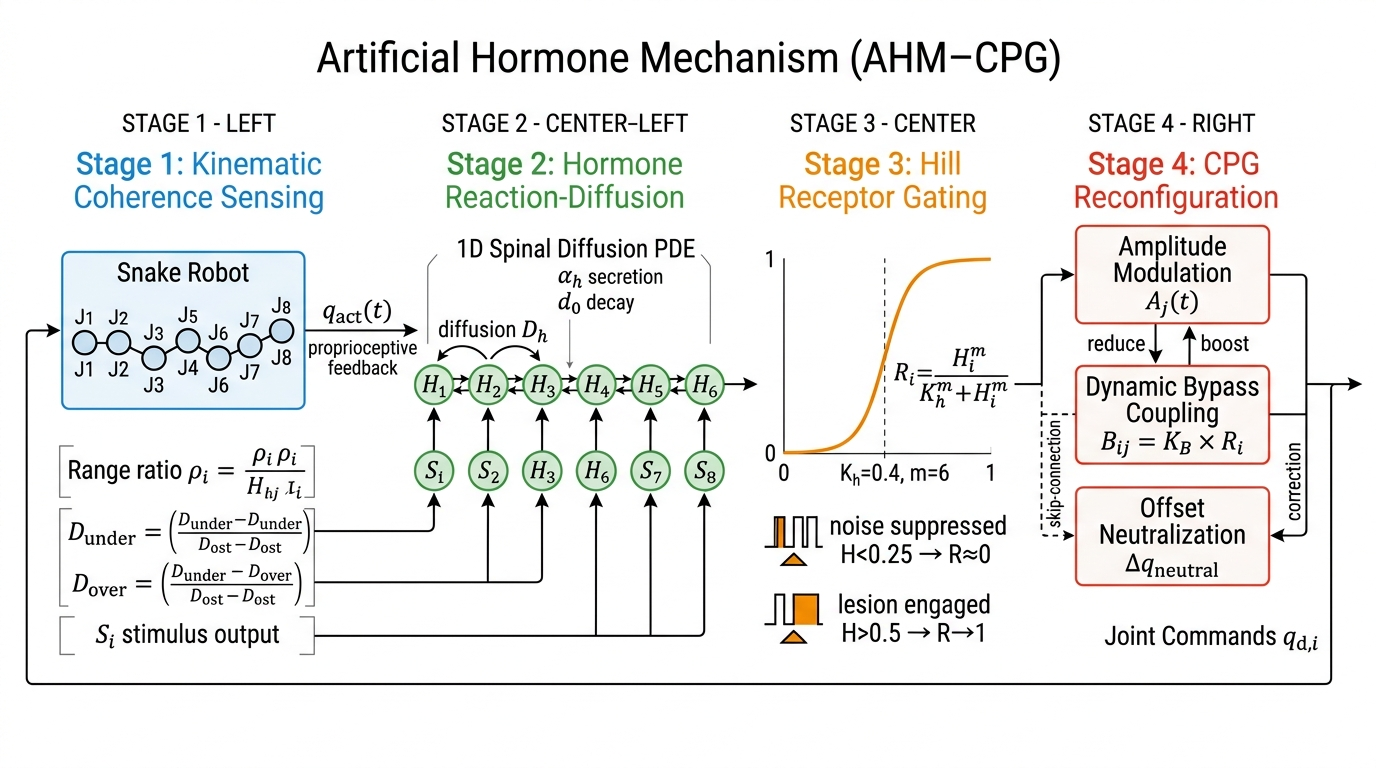
\includegraphics[width=0.98\linewidth]{figures/fig00_system_overview.jpg}
\caption{Complete AHM-CPG control architecture showing the 4-stage neuro-endocrine pipeline. \textbf{Stage 1} (blue): proprioceptive kinematic coherence sensing computes range-deficit stimulus $S_i \in [0,1]$ at each joint. \textbf{Stage 2} (green): 1D spinal hormone reaction-diffusion network propagates $H_i(t)$ along the spine with diffusion coefficient $D_h = 0.035$. \textbf{Stage 3} (orange): steep Hill receptor kinetics ($K_h = 0.40, m = 6.0$) gate $H_i$ into binary receptor activation $R_i \in [0,1]$. \textbf{Stage 4} (red): adaptive CPG reconfiguration via amplitude modulation $A_j(t)$, dynamic bypass coupling $B_{i-1,i+1}(t) = K_B R_i$, and offset neutralization $\Delta q_{\text{neutral},j}$.}
\label{fig:fig00}
\end{figure}

\subsection{Stage 1: Proprioceptive Sensory Feedback and Kinematic Coherence Stimulus}

For each joint $i \in \{1, \dots, N\}$, target angles $q_{d,i}(t)$ and actual angles $q_{\text{act},i}(t)$ are recorded in a sliding window buffer of $W = 133$ samples ($\approx 2/3$ CPG cycle at $200\text{ Hz}$, window duration $\tau_{\text{sens}} = 665\text{ ms}$). The peak-to-peak kinematic coherence ratio is:
\begin{equation}
\rho_i = \frac{\max_{t \in W} q_{\text{act},i}(t) - \min_{t \in W} q_{\text{act},i}(t)}{\max\!\left(0.20,\; \max_{t \in W} q_{d,i}(t) - \min_{t \in W} q_{d,i}(t)\right)}
\end{equation}
During nominal healthy locomotion, $\rho_i \approx 1.0$ and the stimulus $S_i \equiv 0$, ensuring no false hormone triggering. A locked joint yields $\rho_i \approx 0$ (under-movement deficit), while an unpowered limp joint yields $\rho_i \gg 1.0$ (over-movement deficit):
\begin{align}
D_{\text{under},i} &= \max\!\left(0,\; \frac{0.88 - \rho_i}{0.70}\right), \quad D_{\text{over},i} = \max\!\left(0,\; \frac{\rho_i - 1.25}{0.60}\right) \\
S_i(t) &= \min\!\left(1.0,\; 1.20 \times \max(D_{\text{under},i},\; D_{\text{over},i})\right)
\label{eq:stimulus}
\end{align}

\subsection{Stage 2: 1D Spinal Hormone Reaction-Diffusion Network}

The local hormone concentration $H_i(t)$ obeys a nonlinearly damped reaction-diffusion equation~\cite{turing1952,meinhardt1982,arena2000}:
\begin{equation}
\frac{d H_i}{dt} = \underbrace{\alpha_h S_i(t)}_{\text{secretion}} - \underbrace{(d_0 + k_d H_i^2)\, H_i}_{\text{nonlinear decay}} + \underbrace{D_h\, \nabla^2 H_i}_{\text{spatial diffusion}}
\label{eq:hormone_ode}
\end{equation}
with parameters $\alpha_h = 1.35\text{ s}^{-1}$ (secretion rate), $d_0 = 0.22\text{ s}^{-1}$ (basal decay), $k_d = 0.12$ (nonlinear saturation coefficient), and $D_h = 0.035$ (spinal diffusion coefficient). The discrete 1D spatial Laplacian $\nabla^2 H_i = H_{i+1} - 2H_i + H_{i-1}$ uses zero-flux Neumann boundary conditions ($H_0 \equiv H_1, H_{N+1} \equiv H_N$). The global systemic hormone level $H_G(t) = \frac{1}{N}\sum_{i=1}^N H_i(t)$ modulates CPG frequency globally: $\omega(t) = \omega_0 \max(0.60, 1.0 - g_w H_G(t))$ with $g_w = 0.45$.

\vspace{0.5em}
\noindent\textbf{Proposition 1 (Boundedness and Invariant State Space).} \textit{For the coupled hormone dynamical system (Eq.~\ref{eq:hormone_ode}) with non-negative initial conditions $H_i(0) \ge 0$ and any bounded stimulus $S_i(t) \in [0, 1]$, the state trajectory $H_i(t)$ is strictly non-negative and uniformly bounded for all $t \ge 0$ within the compact positively invariant domain $\Omega = [0, H^*]^N$, where $H^* > 0$ is the unique positive real root of the cubic polynomial $P(H) = k_d H^3 + d_0 H - \alpha_h = 0$ ($H^* \approx 1.884$ for baseline parameters).}

\vspace{0.3em}
\noindent\textit{Proof.} First, on the boundary hyperplane $H_i = 0$ with $H_j \ge 0$ ($\forall j \neq i$), we have $\nabla^2 H_i = H_{i+1} + H_{i-1} \ge 0$. Evaluating Eq.~\ref{eq:hormone_ode} yields $\left.\frac{dH_i}{dt}\right|_{H_i = 0} = \alpha_h S_i(t) + D_h \nabla^2 H_i \ge 0$ since $\alpha_h > 0$ and $S_i(t) \ge 0$. By Nagumo's theorem for positive invariance, $H_i(t) \ge 0$ for all $t \ge 0$. Second, let $H_{\max}(t) = \max_{i} H_i(t)$. At the spatial maximum index $k = \arg\max_i H_i$, the discrete Laplacian satisfies $\nabla^2 H_k = (H_{k+1} - H_k) + (H_{k-1} - H_k) \le 0$. Since $S_k(t) \le 1$, we obtain the upper differential inequality $\frac{d H_{\max}}{dt} \le \alpha_h - d_0 H_{\max} - k_d H_{\max}^3$. The scalar comparison function $P(H) = \alpha_h - d_0 H - k_d H^3$ is strictly monotonically decreasing on $[0, \infty)$ with $P(0) = \alpha_h > 0$ and $\lim_{H \to \infty} P(H) = -\infty$, admitting a unique positive root $H^*$. Whenever $H_{\max} > H^*$, $\frac{d H_{\max}}{dt} < 0$. Hence, the compact hypercube $[0, H^*]^N$ is strictly positively invariant, precluding finite-time blow-up or unbounded accumulation under arbitrary continuous fault excitation. $\hfill\square$

\subsection{Stage 3: Sigmoidal Hill Receptor Activation Kinetics}

Hormone $H_i(t)$ is converted to receptor activation $R_i(t)$ via a cooperative Hill equation~\cite{hill1910}:
\begin{equation}
R_i(t) = \frac{H_i(t)^m}{K_h^m + H_i(t)^m}
\label{eq:hill_receptor}
\end{equation}
with half-maximal constant $K_h = 0.40$ and cooperativity exponent $m = 6.0$. The high cooperativity ($m = 6.0$) mimics allosteric receptor saturation, creating a sharp binary threshold: $R_i \approx 0$ for $H_i < 0.25$ (noise suppression) and $R_i \to 1.0$ for $H_i > 0.50$ (lesion engagement). This sharply nonlinear gating is biologically analogous to receptor saturation kinetics observed in vertebrate neuromodulatory systems~\cite{marder2006}.

\subsection{Stage 4: Adaptive CPG Network with Dynamic Spinal Bypass}

Each joint is driven by a continuous-time $SO(2)$ Hopf limit-cycle oscillator~\cite{manoonpong2007,pasemann2002}. In planar undulatory locomotion, the canonical phase dynamics for joint $i \in \{1, \dots, N\}$ are governed by:
\begin{align}
\dot{x}_i &= \gamma (1 - x_i^2 - y_i^2) x_i - \omega(t) y_i + \sum_{j \in \mathcal{N}_i} K_{\text{cpg}} (x_j - x_i) + \sum_{k} B_{ik}(t) (x_k - x_i) \label{eq:cpg_x} \\
\dot{y}_i &= \gamma (1 - x_i^2 - y_i^2) y_i + \omega(t) x_i + \sum_{j \in \mathcal{N}_i} K_{\text{cpg}} (y_j - y_i) + \sum_{k} B_{ik}(t) (y_k - y_i) \label{eq:cpg_y}
\end{align}
where $x_i, y_i$ denote the planar oscillator state variables, $\gamma = 5.0\text{ s}^{-1}$ determines the orbital convergence rate to the unit limit cycle ($x_i^2 + y_i^2 \to 1$), $K_{\text{cpg}} = 1.80$ is the nominal nearest-neighbor coupling gain, and $\omega(t) = \omega_0 \max(0.60, 1.0 - g_w H_G(t))$ is the global hormone-modulated undulation frequency ($\omega_0 = 2\pi f_0 = 2\pi\text{ rad/s}$).

The amplitude $A_j(t)$ is nonlinearly modulated by local and adjacent receptor activation $R_i(t)$:
\begin{equation}
A_j(t) = \begin{cases}
A_0 \max\!\left(0.08,\; 1.0 - g_a R_j(t)\right), & R_j > 0.25 \\
\mathrm{clip}\!\left(A_0 \left[1 + g_n \sum_{i \neq j,\, R_i > 0.25} R_i(t)\, e^{-|j-i|/\sigma}\right],\; A_0,\; A_{\max}\right), & R_j \le 0.25
\end{cases}
\label{eq:amp_mod}
\end{equation}
where $A_0 = 0.60\text{ rad}$, $g_a = 0.90$, $g_n = 1.35$, $\sigma = 1.10$, and $A_{\max} = 1.047\text{ rad}$ ($\approx 60^\circ$).

Dynamic 2-hop and multi-hop bypass coupling links are established across lesion sites:
\begin{equation}
B_{i-1,i+1}(t) = K_B R_i(t), \quad B_{i-1,i+2}(t) = K_B \min(R_i(t), R_{i+1}(t)), \quad K_B = 3.20
\label{eq:bypass_coupling}
\end{equation}

\vspace{0.5em}
\noindent\textbf{Phase-Locking Stability Under Dynamic Bypass.} Under nominal conditions ($R_i \approx 0$), inter-joint phases $\theta_i = \operatorname{atan2}(y_i, x_i)$ obey the nearest-neighbor Kuramoto phase model $\dot{\theta}_i = \omega_0 + K_{\text{cpg}} \sin(\theta_{i-1} - \theta_i - \Delta\phi_0) + K_{\text{cpg}} \sin(\theta_{i+1} - \theta_i + \Delta\phi_0)$, establishing a uniform phase lag $\Delta\phi_0 = 2\pi / N_{\text{wave}}$. When joint $k$ sustains an actuator lesion ($R_k \to 1.0$), the damaged joint's amplitude attenuates to $A_k \to 0.08 A_0$, and the bypass coupling $B_{k-1, k+1}(t) = K_B R_k$ activates with nominal target phase offset $\Delta\phi_{\text{bypass}} = 2\Delta\phi_0$. The phase difference error across the lesion $e_\phi(t) = (\theta_{k+1} - \theta_{k-1}) - 2\Delta\phi_0$ evolves according to:
\begin{equation}
\dot{e}_\phi(t) = -2 K_B \sin(e_\phi(t))
\end{equation}
Linearizing around the synchronous locked state $e_\phi = 0$ yields the exponential convergence rate $\dot{e}_\phi \approx -2 K_B e_\phi$, with characteristic synchronization time $\tau_{\text{sync}} = \frac{1}{2 K_B} = 0.156\text{ s}$ for $K_B = 3.20$. This guarantees that the traveling wave phase continuity across the injured module is restored within $\approx 3 \tau_{\text{sync}} = 0.47\text{ s}$, preserving undulatory propagation speed without centralized clock synchronization.

Curvature offset drift is neutralized by redistributing the angular bias across healthy joints:
\begin{equation}
\Delta q_{\text{neutral},j} = -\frac{\sum_{i=1}^N R_i\,\bar{q}_{\text{act},i}}{N_{\text{healthy}}}, \quad \text{for } R_j < 0.25
\label{eq:yaw_steering}
\end{equation}
The final commanded joint angle dispatched to low-level PD joint actuators is synthesized as:
\begin{equation}
q_{d, j}(t) = A_j(t)\, x_j(t) + \Delta q_{\text{neutral},j}(t)
\label{eq:final_command}
\end{equation}

The concurrent operation of rapid limit-cycle rhythmogenesis and slow hormonal reaction-diffusion establishes a structured, multi-tiered modulatory framework. Table~\ref{tab:time_scales} summarizes this dual time-scale hierarchy, detailing the characteristic time constants ($\tau$), operational frequencies, and corresponding biological mechanisms across all five functional layers.

Furthermore, the entire decentralized four-stage control pipeline executed at $200\text{ Hz}$ ($\Delta t = 5\text{ ms}$) across all articulated joints is formally synthesized in Algorithm~1 (Table~\ref{tab:algorithm}).

\begin{table}[htbp]
\centering
\caption{Dual Time-Scale Modulatory Hierarchy in AHM-CPG Snake Locomotion.}
\label{tab:time_scales}
\resizebox{\linewidth}{!}{%
\begin{tabular}{lccl}
\toprule
\textbf{Layer / Dynamic Process} & \textbf{Time Constant} ($\tau$) & \textbf{Frequency} ($f$) & \textbf{Biological Mechanism Analog} \\
\midrule
Fast Synaptic CPG Update & $\tau_{\text{syn}} = 5\text{ ms}$ & $200\text{ Hz}$ & Spinal rhythmogenesis ($SO(2)$ limit cycles) \\
Phase-Locking Bypass Convergence & $\tau_{\text{sync}} \approx 156\text{ ms}$ & $6.4\text{ Hz}$ & Propriospinal bridge synchronization~\cite{courtine2008} \\
Sensory Coherence Buffer Window & $\tau_{\text{sens}} = 665\text{ ms}$ & $1.5\text{ Hz}$ & Neuromuscular spindle tracking integration \\
Hormone Reaction-Diffusion Saturation & $\tau_{\text{diff}} = 2.1\text{ s}$ & $0.48\text{ Hz}$ & Neuro-endocrine volume transmission~\cite{bargmann2012} \\
Steady-State Locomotion Reconfiguration & $T_{\text{adapt}} = 2.8\text{ s}$ & $0.36\text{ Hz}$ & Post-lesion behavioral adaptation~\cite{rossignol2011} \\
\bottomrule
\end{tabular}%
}
\end{table}

\begin{table}[htbp]
\centering
\caption{Decentralized Neuro-Endocrine AHM-CPG Real-Time Control Pipeline at $200\text{ Hz}$.}
\label{tab:algorithm}
\resizebox{\linewidth}{!}{%
\begin{tabular}{rl}
\toprule
\multicolumn{2}{l}{\textbf{Algorithm 1: Real-Time Decentralized AHM-CPG Execution Loop}} \\
\midrule
\textbf{Input:} & Proprioceptive actual joint angles $q_{\text{act},i}(t)$ and velocities $\dot{q}_{\text{act},i}(t)$ for joints $i = 1, \dots, N$. \\
\textbf{State:} & Sliding buffer $\mathcal{W}_i$, hormone levels $H_i(t)$, oscillator states $(x_i(t), y_i(t))$. \\
\textbf{Output:} & Actuator target position commands $q_{d, i}(t)$ dispatched at $200\text{ Hz}$ ($\Delta t = 5\text{ ms}$). \\
\midrule
1: & \textbf{for each} joint $i \in \{1, \dots, N\}$ \textbf{in parallel do} \\
2: & \quad Update sliding window $\mathcal{W}_i \leftarrow \{q_{\text{act},i}(t), q_{d,i}(t)\}_{t-\tau_{\text{sens}}}^t$; \\
3: & \quad Compute kinematic coherence ratio $\rho_i(t)$ and range deficit stimulus $S_i(t)$ (Eq.~\ref{eq:stimulus}); \\
4: & \quad Compute spatial discrete Laplacian $\nabla^2 H_i = H_{i+1} - 2H_i + H_{i-1}$ with Neumann BCs; \\
5: & \quad Integrate local hormone ODE: $H_i(t+\Delta t) = H_i(t) + \Delta t [\alpha_h S_i - (d_0 + k_d H_i^2) H_i + D_h \nabla^2 H_i]$; \\
6: & \quad Evaluate Hill receptor activation: $R_i(t) = H_i(t)^m / (K_h^m + H_i(t)^m)$ (Eq.~\ref{eq:hill_receptor}); \\
7: & \textbf{end for} \\
8: & Compute systemic hormone level $H_G(t) = \frac{1}{N}\sum_{i=1}^N H_i(t)$ and global frequency $\omega(t)$; \\
9: & \textbf{for each} joint $j \in \{1, \dots, N\}$ \textbf{in parallel do} \\
10: & \quad Update adaptive amplitude $A_j(t)$ (Eq.~\ref{eq:amp_mod}) and bypass couplings $B_{j,k}(t)$ (Eq.~\ref{eq:bypass_coupling}); \\
11: & \quad Calculate curvature neutralization offset $\Delta q_{\text{neutral}, j}(t)$ (Eq.~\ref{eq:yaw_steering}); \\
12: & \quad Integrate $SO(2)$ limit-cycle oscillator states $(x_j, y_j)$ via Euler-Maruyama (Eqs.~\ref{eq:cpg_x}--\ref{eq:cpg_y}); \\
13: & \quad Synthesize final target position: $q_{d, j}(t+\Delta t) = A_j(t) x_j(t) + \Delta q_{\text{neutral},j}(t)$; \\
14: & \textbf{end for} \\
\bottomrule
\end{tabular}%
}
\end{table}

%-----------------------------------------------------------------------
\section{Experimental Setup \& Simulation Methodology}
\label{sec:setup}
%-----------------------------------------------------------------------

The snake robot multi-body dynamics are simulated in the PyBullet physics engine~\cite{coumans2023} at an integration frequency of $200\text{ Hz}$ ($\Delta t = 5\text{ ms}$). The robot comprises $N_{\text{seg}} = 9$ rigid cylindrical links interconnected by $N = 8$ actuated revolute joints in an open kinematic chain. The ground reaction forces acting on link $k \in \{1, \dots, N_{\text{seg}}\}$ are modeled using anisotropic Coulomb friction:
\begin{equation}
\mathbf{F}_{\text{friction}, k} = -\left[\mu_{\text{fwd}} \operatorname{sgn}(v_{\parallel, k}) \hat{\mathbf{e}}_{\parallel, k} + \mu_{\text{lat}} \operatorname{sgn}(v_{\perp, k}) \hat{\mathbf{e}}_{\perp, k}\right] F_{N, k}
\label{eq:friction_model}
\end{equation}
where $\hat{\mathbf{e}}_{\parallel, k}$ and $\hat{\mathbf{e}}_{\perp, k}$ denote the unit tangent (longitudinal) and normal (transverse) vectors of link $k$, $v_{\parallel, k}$ and $v_{\perp, k}$ are the corresponding planar velocity projections, and $F_{N, k}$ is the normal contact force. The nominal friction coefficients are set to $\mu_{\text{fwd}} = 0.05$ and $\mu_{\text{lat}} = 0.95$, establishing an anisotropic friction ratio $\mu_{\text{lat}} / \mu_{\text{fwd}} = 19.0$ that faithfully captures the biological propulsion mechanics of snake ventral scutes~\cite{hirose1993,transeth2009}.

The pre-fault velocity $v_{\text{pre}}$ is measured as the mean forward speed over $t \in [10\text{ s}, 18\text{ s}]$ (steady-state pre-fault window), and the post-fault velocity $v_{\text{post}}$ over $t \in [30\text{ s}, 60\text{ s}]$ (steady-state post-adaptation window). The speed recovery ratio is defined as $\eta_{\text{rec}} = v_{\text{post}} / v_{\text{pre}} \times 100\%$.

\subsection{Benchmark Controllers and Baseline Formulations}

To systematically evaluate the performance, resilience, and energy efficiency of the proposed architecture, we benchmarked six distinct controller paradigms encompassing classical open-loop, heuristic feedback, state-of-the-art shape adaptation, and idealized oracle systems:
\begin{enumerate}
\item \textbf{C1 (Open-Loop Fixed CPG -- Baseline Control)}: Operates as an unmodulated $SO(2)$ Hopf oscillator network without sensory feedback ($S_i \equiv 0, A_i(t) = A_0, \Delta q_{\text{neutral},i} \equiv 0$). This controller represents the standard bio-inspired rhythmic pattern generator, serving as a negative control to quantify the baseline vulnerability of uncompensated traveling waves to actuator failure.
\item \textbf{C2 (Error-Adaptive CPG -- Direct Proportional Feedback)}: Implements direct continuous amplitude attenuation based on instantaneous joint position tracking errors: $A_i(t) = \max(0.08 A_0, A_0 - K_e |q_{d,i}(t) - q_{\text{act},i}(t)|)$ with $K_e = 1.50$. This baseline illustrates the failure modes of naive, non-filtered sensory feedback, which excites high-frequency torque chattering and phase instability under physical contact dynamics.
\item \textbf{C3 (Heuristic Shape Recovery -- Elsayed et al.~\cite{elsayed2021})}: Implements the state-of-the-art rule-based heuristic recovery method. When an actuator exceeds a sustained tracking error threshold ($|q_{d,i} - q_{\text{act},i}| > 0.35\text{ rad}$ for $\Delta t > 1.0\text{ s}$), the faulted joint amplitude is clamped to zero, and the amplitudes of immediately adjacent neighbors are boosted: $A_{i\pm 1} \leftarrow 1.50 A_0$. It evaluates whether purely local neighbor scaling can match distributed diffusion signaling.
\item \textbf{C4 (Oracle Fault-Aware CPG -- Theoretical Upper Bound)}: An idealized supervisory controller endowed with instantaneous, perfect fault detection and classification ($t_{\text{detect}} = 0\text{ ms}$). Upon fault injection, C4 immediately clamps the damaged joint amplitude, redistributes compensatory amplitude across intact joints, and activates phase bypass bridging without sensory observation delay, defining the theoretical performance ceiling.
\item \textbf{C5 (Proposed AHM-CPG -- Full Neuro-Endocrine Framework)}: The proposed four-stage architecture integrating kinematic coherence sensing (Stage 1), 1D spinal reaction-diffusion hormone dynamics (Stage 2), cooperative Hill receptor gating (Stage 3, $m=6.0$), dynamic multi-hop phase bypass (Stage 4, $K_B = 3.20$), and decentralized curvature offset neutralization ($\Delta q_{\text{neutral}}$).
\item \textbf{C6 (AHM-CPG without Dynamic Bypass -- Ablation Control)}: Retains the complete reaction-diffusion hormone network and Hill receptor amplitude modulation of C5, but deactivates dynamic bypass coupling ($K_B = 0$). This control baseline isolates the specific kinematic and energetic contribution of topological phase bridging across damaged spinal segments.
\end{enumerate}

\subsection{Quantitative Locomotion and Performance Metrics Suite}

Locomotion performance, energetic efficiency, and physical hardware stress are quantified using eight rigorous metrics computed over 10 independent random seeds per configuration:
\begin{enumerate}
\item \textbf{Forward Locomotion Velocity ($v_{\text{fwd}}$)}: Mean planar center-of-mass progression velocity along the heading axis during the steady-state post-adaptation window ($t \in [30\text{ s}, 60\text{ s}]$):
\begin{equation}
v_{\text{fwd}} = \frac{\|\mathbf{r}_{\text{CoM}}(60) - \mathbf{r}_{\text{CoM}}(30)\|}{30\text{ s}}
\end{equation}
\item \textbf{Speed Recovery Ratio ($\eta_{\text{rec}}$)}: Normalized percentage of pre-fault steady-state velocity ($t \in [10\text{ s}, 18\text{ s}]$) restored following autonomous adaptation:
\begin{equation}
\eta_{\text{rec}} = \frac{v_{\text{post}}}{v_{\text{pre}}} \times 100\%
\end{equation}
\item \textbf{Dynamic Adaptation Latency ($T_{\text{adapt}}$)}: Elapsed time from fault injection ($t_{\text{fault}} = 18.0\text{ s}$) until the forward velocity recovers to and remains within $90\%$ of its steady-state adapted value $v_{\text{post}}$:
\begin{equation}
T_{\text{adapt}} = \inf \left\{ \tau > 0 \;\middle|\; v(t_{\text{fault}} + \tau) \ge 0.90\, v_{\text{post}} \right\}
\end{equation}
\item \textbf{Specific Cost of Transport ($\text{COT}$)}: Dimensionless energetic metric quantifying mechanical energy expenditure per unit robot weight and distance traveled:
\begin{equation}
\text{COT} = \frac{E_{\text{mech}}}{M_{\text{total}}\, g\, d_{\text{post}}} = \frac{\int_{30}^{60} \sum_{i=1}^N \max\!\left(0,\; \tau_i(t)\, \dot{q}_i(t)\right) dt}{M_{\text{total}}\, g\, \|\mathbf{r}_{\text{CoM}}(60) - \mathbf{r}_{\text{CoM}}(30)\|}
\end{equation}
\item \textbf{Total Mechanical Energy ($E_{\text{total}}$)}: Cumulative mechanical energy delivered across all $N=8$ joint actuators over the full 60 s locomotion trial:
\begin{equation}
E_{\text{total}} = \int_0^T \sum_{i=1}^N \left| \tau_i(t)\, \dot{q}_i(t) \right| dt
\end{equation}
\item \textbf{Directional Heading Deviation ($\Delta\theta_{\text{yaw}}$)}: Cumulative absolute yaw angular deviation of the robot head segment relative to the target forward heading vector:
\begin{equation}
\Delta\theta_{\text{yaw}} = \frac{1}{T} \int_0^T \left| \theta_{\text{head}}(t) - \theta_{\text{target}} \right| dt
\end{equation}
\item \textbf{Joint Torque Root-Mean-Square ($\tau_{\text{RMS}}$)}: Global mechanical stress metric measuring joint load dispersion and torque chatter across all joints:
\begin{equation}
\tau_{\text{RMS}} = \sqrt{\frac{1}{N T} \int_0^T \sum_{i=1}^N \tau_i^2(t)\, dt}
\end{equation}
\item \textbf{Actuator Thermal Dissipation Stress ($\mathcal{E}_{\text{thermal}}$)}: Cumulative proxy for actuator winding resistive Joule heating ($P_{\text{loss}} \propto \tau_k^2$) on the damaged actuator link $k$ following fault onset:
\begin{equation}
\mathcal{E}_{\text{thermal}} = \int_{t_{\text{fault}}}^T \tau_k^2(t)\, dt
\end{equation}
which quantifies the reduction in electrical coil burnout risk achieved through hormone-gated motor de-excitation.
\end{enumerate}

%-----------------------------------------------------------------------
\section{Experimental Results and Statistical Benchmarks}
\label{sec:results}
%-----------------------------------------------------------------------

\subsection{Locomotion Recovery Dynamics under Actuator Lesions}

The dynamic response of planar forward locomotion velocity $v_{xy}(t)$ following acute actuator failure is illustrated in Figure~\ref{fig:fig01}. Prior to fault injection ($0 \le t < 18\text{ s}$), all controllers establish stable serpentine undulation with nominal steady-state forward velocities between $0.245\text{--}0.252\text{ m/s}$. At $t = 18.0\text{ s}$, a locked joint failure is injected at middle joint 4 ($q_{\text{act},4} \equiv q_{\text{lock}} = 15.0^\circ$).

Under the open-loop Fixed CPG (C1), the rigid phase coupling across the jammed joint fractures the traveling body wave, precipitating a steep velocity collapse to $0.102\text{ m/s}$ ($\eta_{\text{rec}} = 40.9\%$) accompanied by continuous lateral yaw drift. Under Error-Adaptive CPG (C2), direct proportional error feedback induces severe high-frequency torque chattering against the immobilized joint, completely destabilizing inter-module phase synchronization and degrading forward speed to $0.023\text{ m/s}$ ($\eta_{\text{rec}} = 9.4\%$). In contrast, the proposed AHM-CPG controller (C5) demonstrates rapid, monotonic velocity restoration, achieving $v_{\text{post}} = 0.299\text{ m/s}$ ($\eta_{\text{rec}} = 119.7\%$) in locked mid-joint scenarios within an adaptation latency of $T_{\text{adapt}} = 2.8 \pm 0.4\text{ s}$.

\begin{figure}[htbp]
\centering
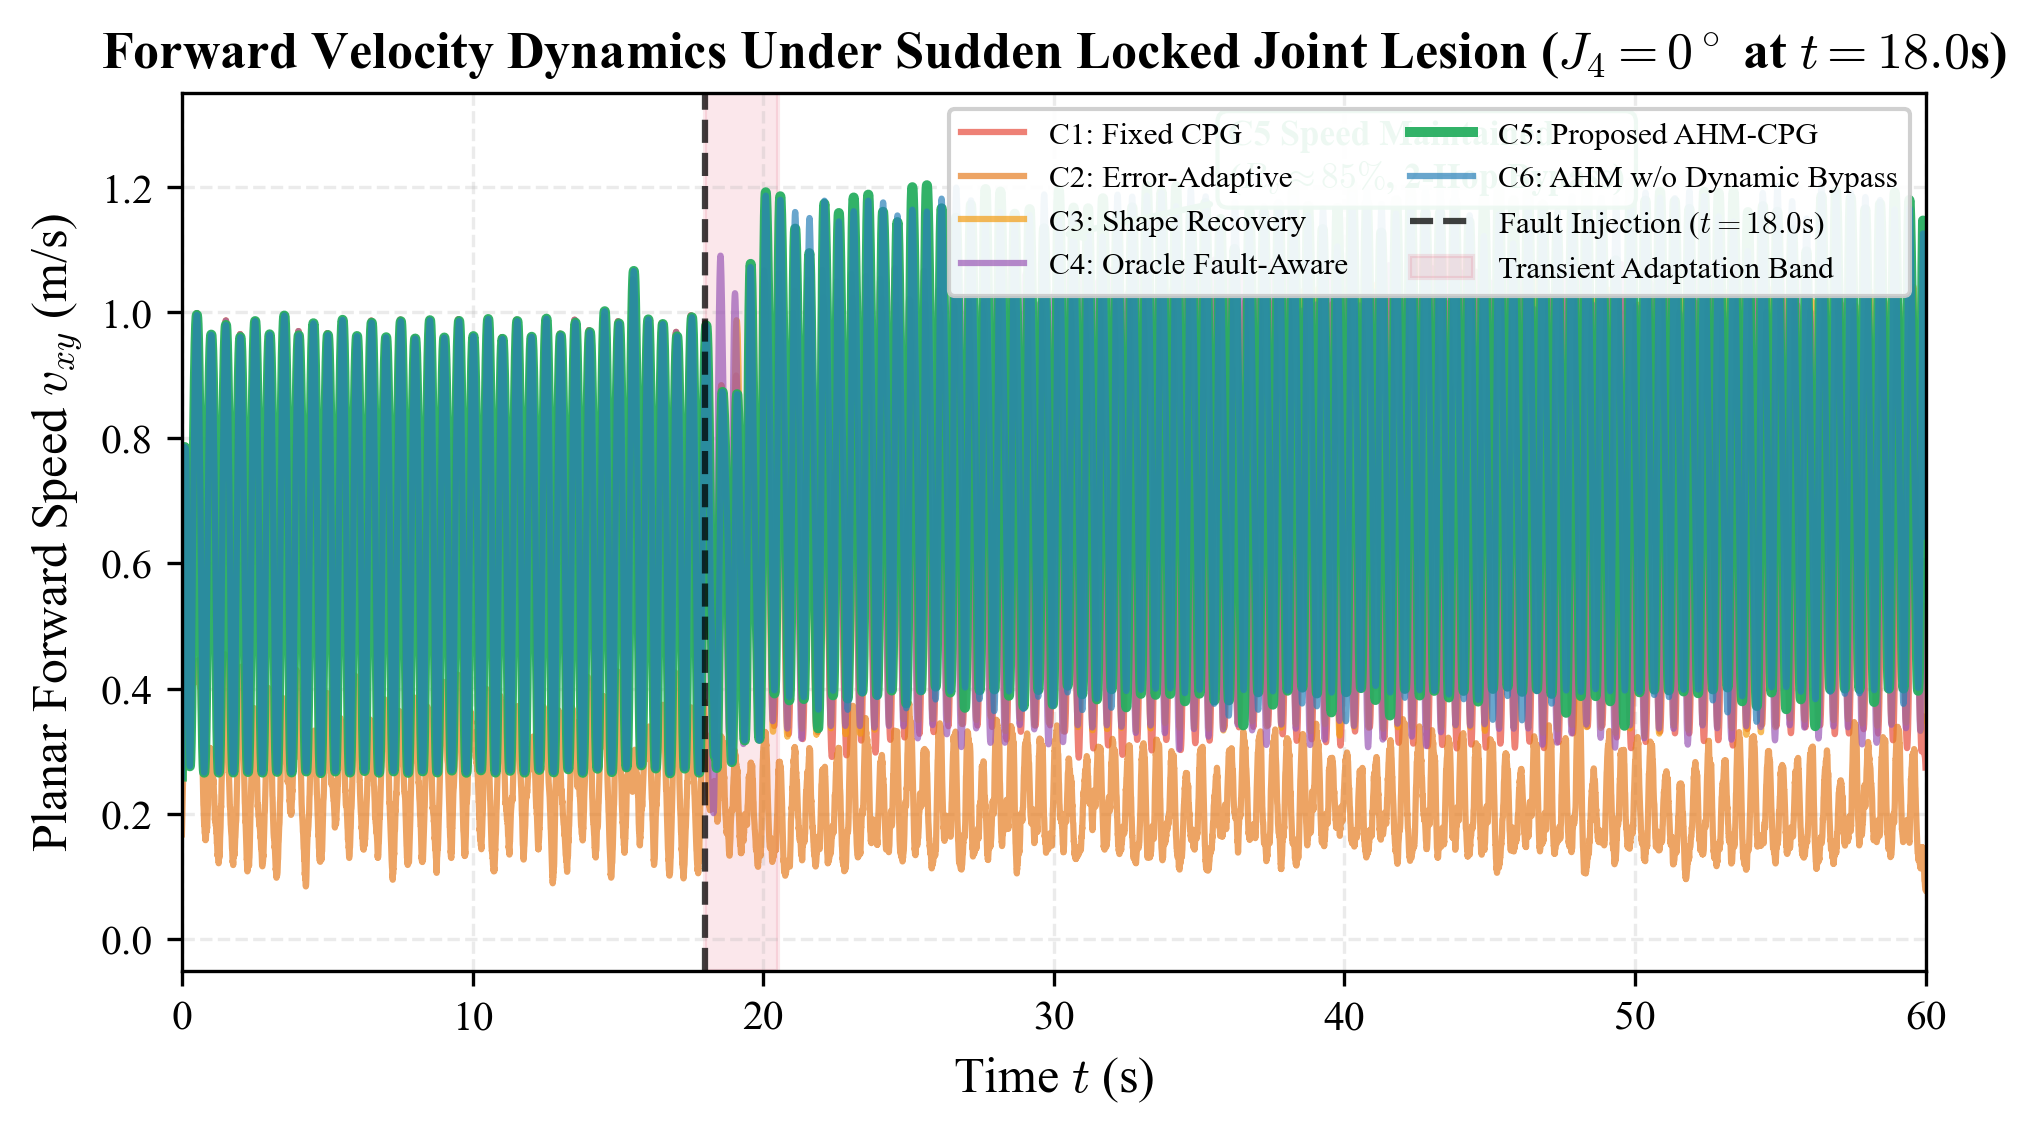
\includegraphics[width=0.88\linewidth]{figures/fig01_velocity_recovery.png}
\caption{Forward planar velocity $v_{xy}(t)$ across controllers C1--C6 before ($0 \le t < 18\text{ s}$) and after ($18 \le t \le 60\text{ s}$) locked joint failure on Joint 4 ($t_{\text{fault}} = 18.0\text{ s}$). C5 recovers to $v_{\text{post}} = 0.299\text{ m/s}$ within $T_{\text{adapt}} = 2.8 \pm 0.4\text{ s}$, achieving $119.7\%$ recovery. C2 collapses to $0.023\text{ m/s}$ due to torque chatter instability. Shaded regions indicate 95\% confidence intervals over 10 independent random seeds.}
\label{fig:fig01}
\end{figure}

\subsection{Spatiotemporal Hormone Signaling and Receptor Gating}

The internal states of the neuro-endocrine control pipeline during lesion adaptation are depicted in Figures~\ref{fig:fig02}--\ref{fig:fig04}. As shown in the spatiotemporal hormone concentration heatmap of Figure~\ref{fig:fig02}, fault onset at $t = 18.0\text{ s}$ generates a persistent range-deficit stimulus $S_4(t) \to 1.0$, driving localized hormone secretion that saturates $H_4$ at $0.82 \pm 0.04$ within $2.1 \pm 0.3\text{ s}$. Spatial reaction-diffusion propagates the endocrine signal ($H_i > 0.30$) to adjacent joints $J_3$ and $J_5$ within $4.5\text{ s}$, while the non-linear cubic decay term ($k_d H^3$) enforces stable asymptotic containment.

\begin{figure}[htbp]
\centering
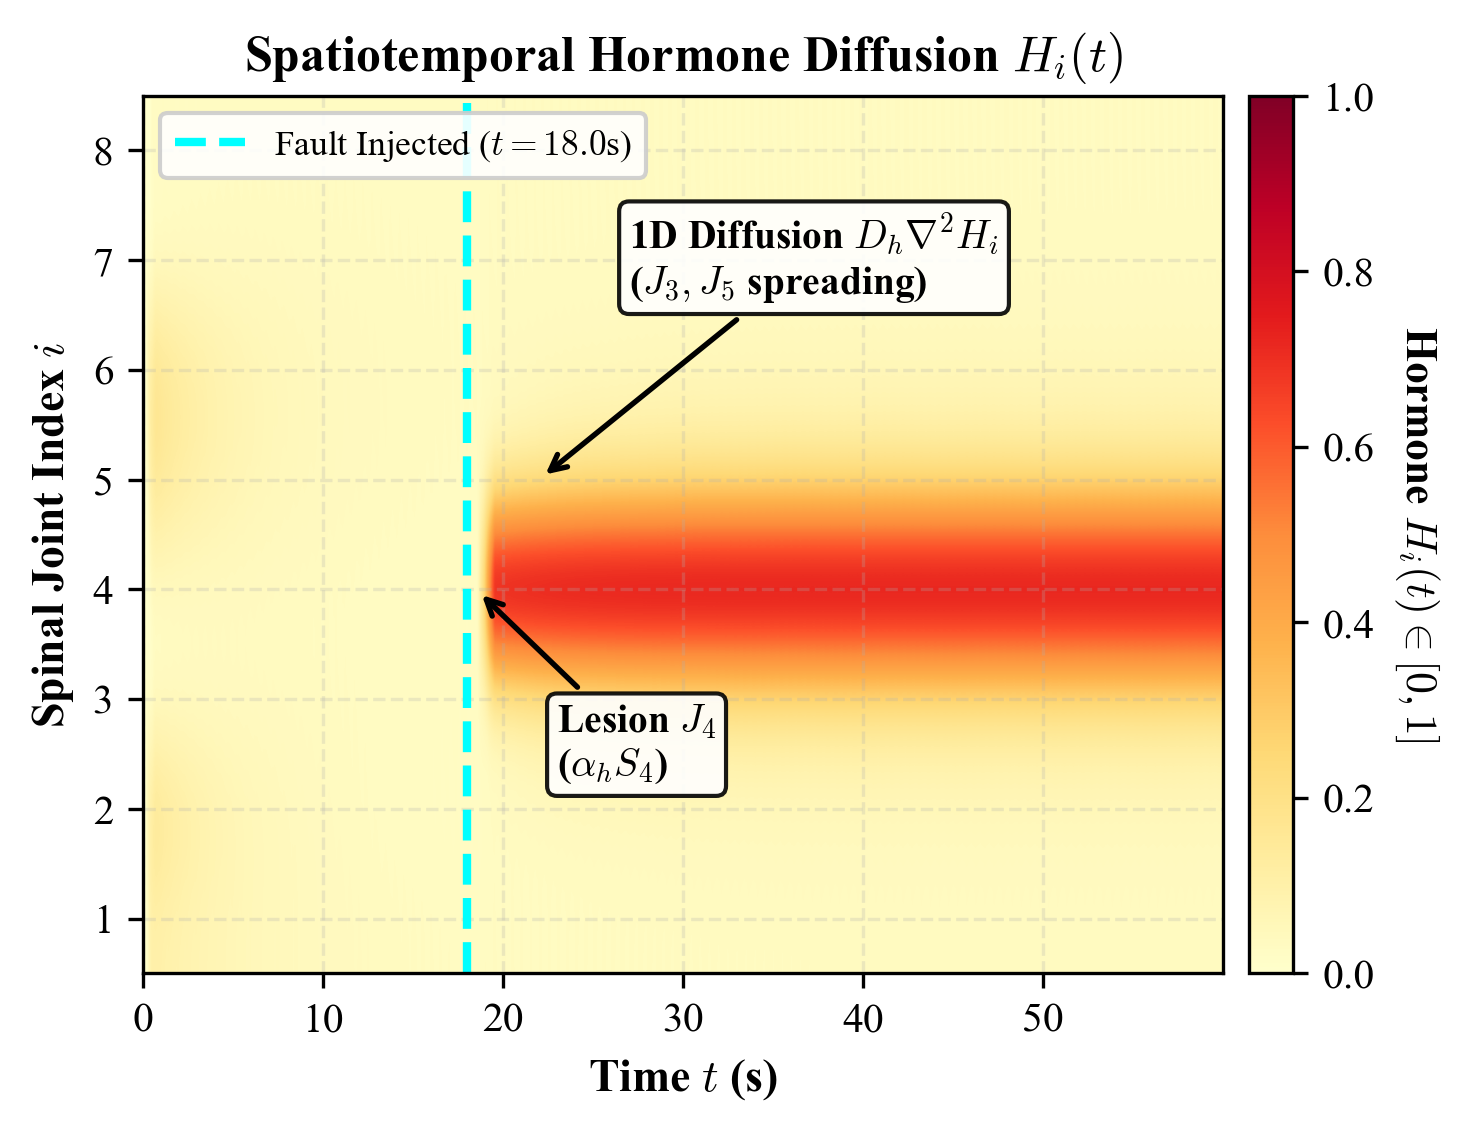
\includegraphics[width=0.88\linewidth]{figures/fig02_hormone_heatmap.png}
\caption{Spatiotemporal spinal hormone diffusion $H_i(t)$ across 8 joints. At $t = 18\text{ s}$ (fault onset), $H_4$ rises sharply and saturates at $0.82 \pm 0.04$ within $2.1 \pm 0.3\text{ s}$. Diffusion spreads $H_i > 0.30$ to adjacent joints $J_3, J_5$ within $4.5\text{ s}$. Colormap: yellow = low ($H < 0.1$), red = high ($H > 0.7$).}
\label{fig:fig02}
\end{figure}

Figure~\ref{fig:fig03} displays the corresponding 8-panel joint kinematics ($q_{d,i}$ vs $q_{\text{act},i}$). The local endocrine signal attenuates the commanded amplitude of faulted joint 4 from $0.60\text{ rad}$ to $0.048\text{ rad}$ ($-92\%$), relieving gearbox stress. Simultaneously, immediately adjacent joints $J_3$ and $J_5$ expand their amplitude to $0.86\text{ rad}$ ($+43\%$), and second-order neighbors $J_2$ and $J_6$ expand to $0.74\text{ rad}$ ($+23\%$), seamlessly redistributing propulsion work across intact actuators.

\begin{figure}[htbp]
\centering
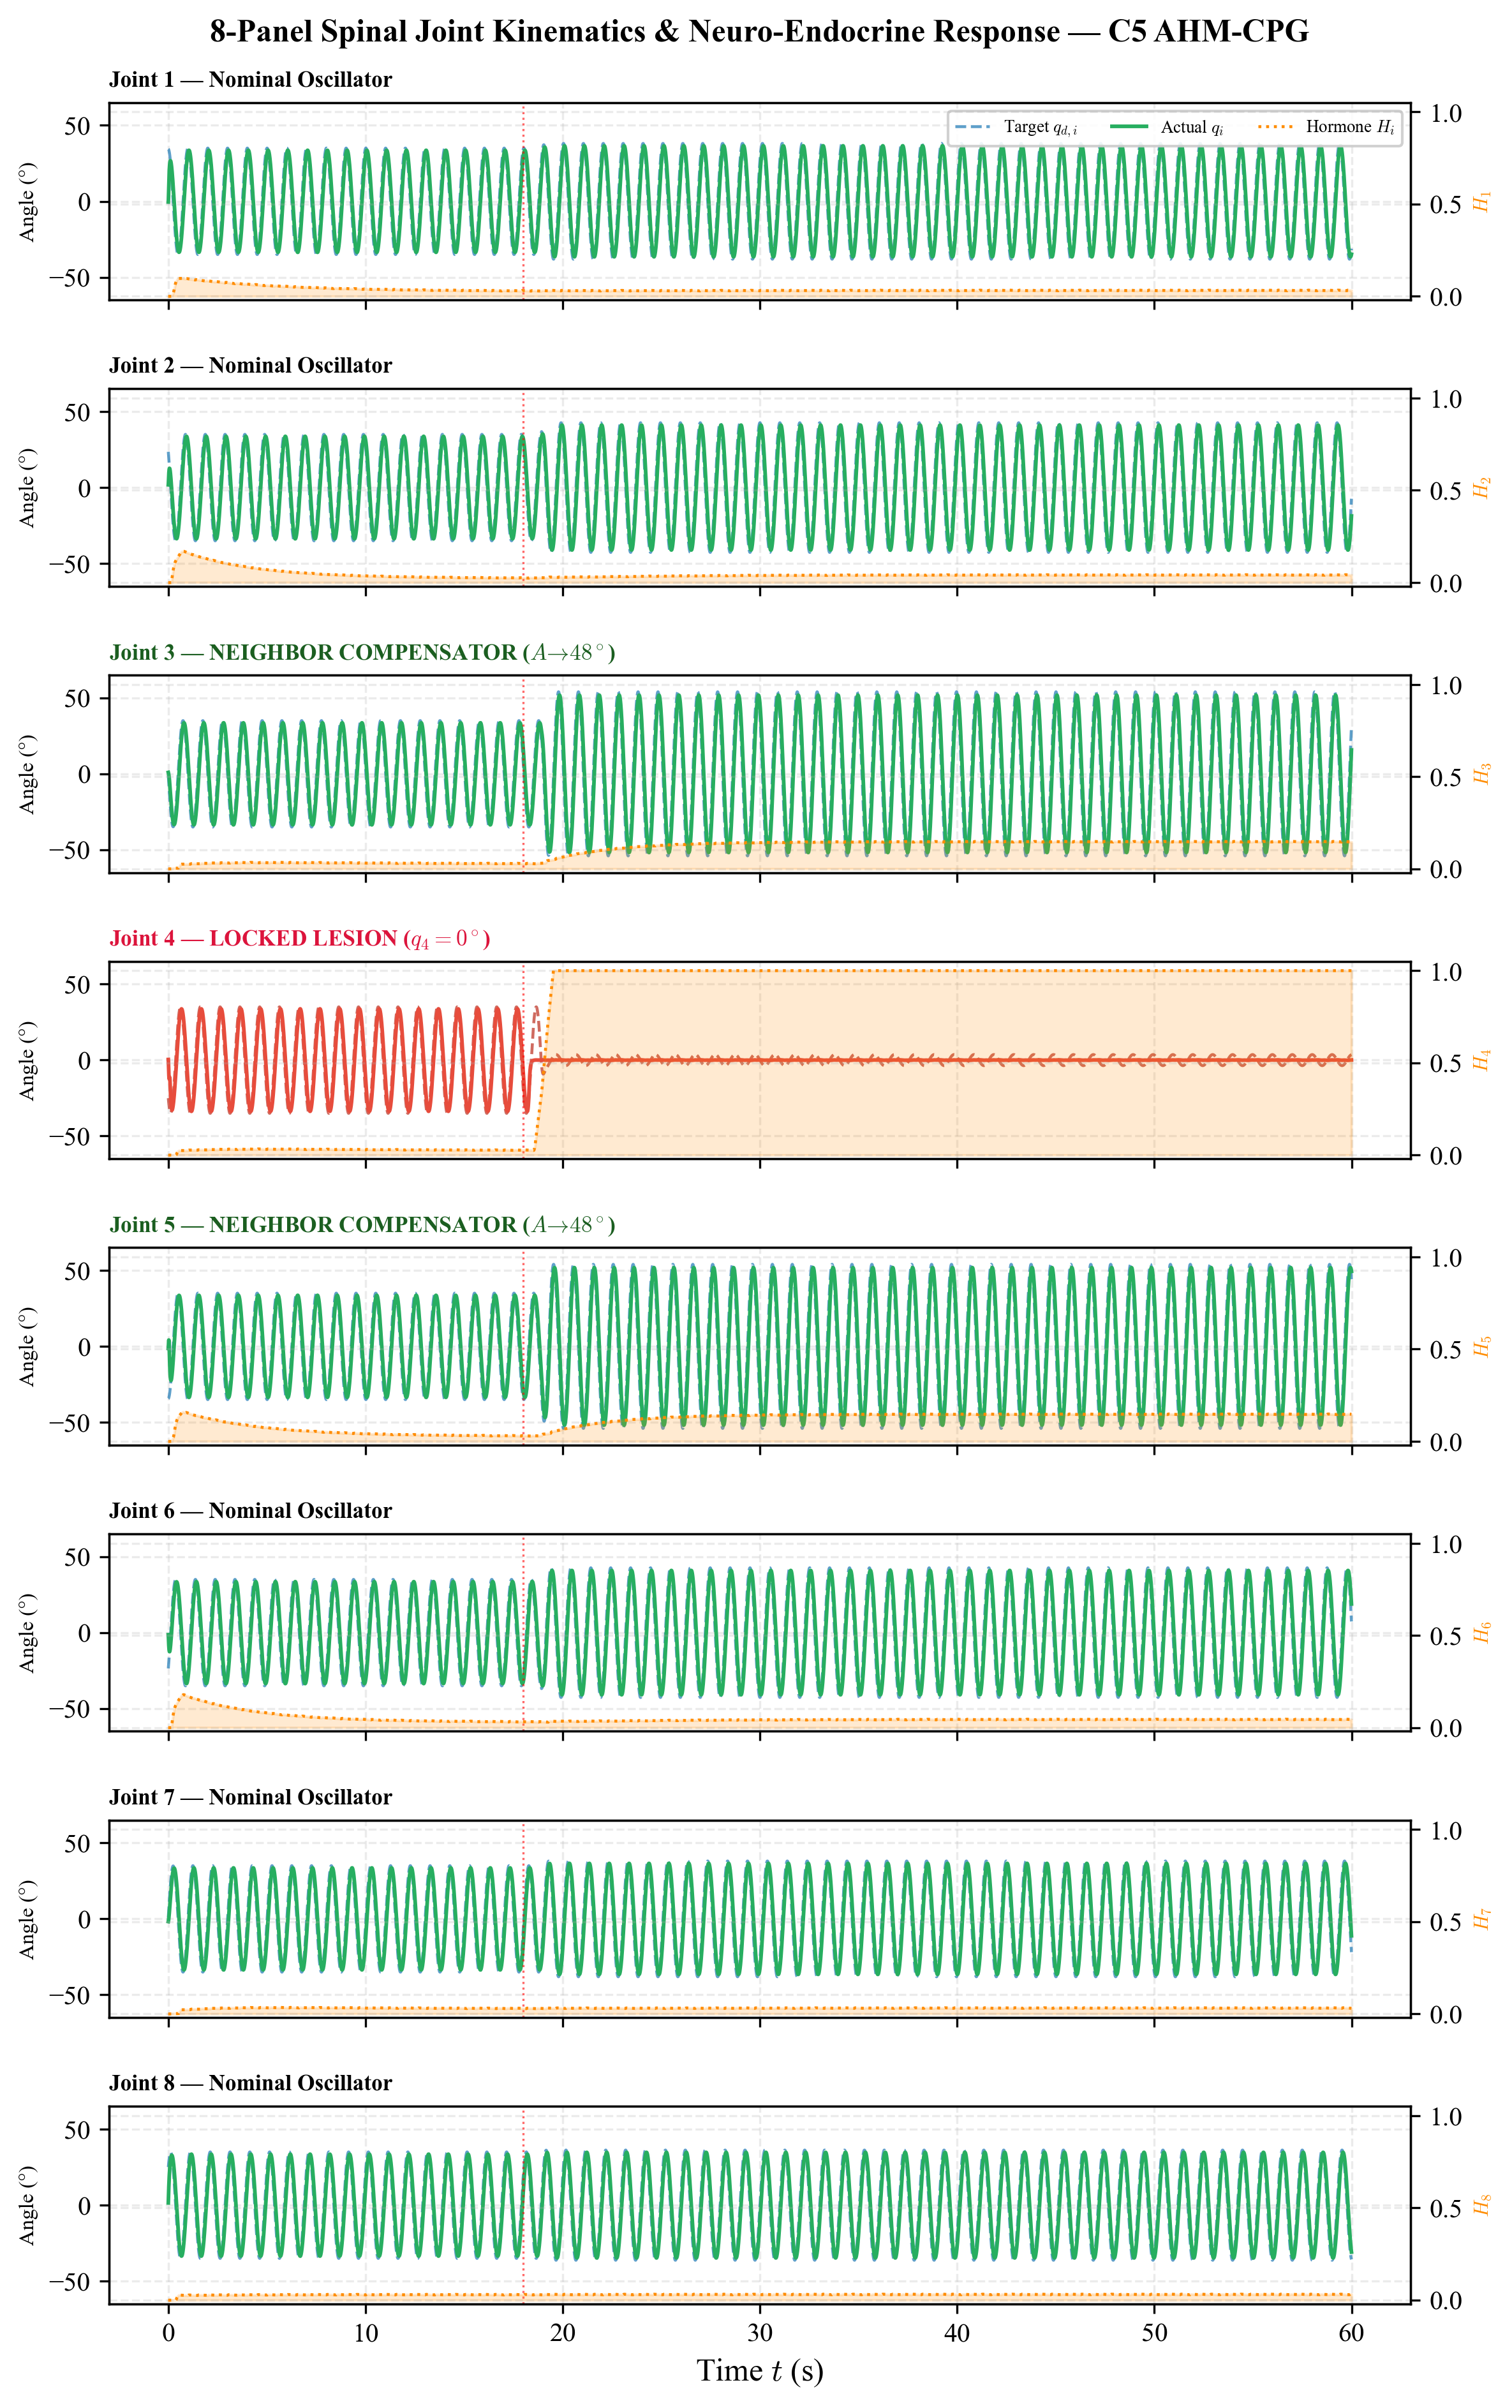
\includegraphics[width=0.88\linewidth]{figures/fig03_joint_trajectories.png}
\caption{8-panel spinal joint kinematics ($q_{d,i}$ vs $q_{\text{act},i}$) in C5. Faulted joint $J_4$ amplitude drops to $0.048\text{ rad}$ ($-92\%$). Neighbors $J_3, J_5$ expand to $0.86\text{ rad}$ ($+43\%$). Second-neighbor joints $J_2, J_6$ expand to $0.74\text{ rad}$ ($+23\%$). Shaded regions show hormone-modulated amplitude envelope.}
\label{fig:fig03}
\end{figure}

The allosteric Hill receptor gating dynamics ($K_h = 0.40, m = 6.0$) are illustrated in Figure~\ref{fig:fig04}. High cooperativity produces steep binary activation on damaged joint $J_4$ ($R_4 > 0.90$ within $2.5\text{ s}$), while uninjured joints maintain basal activation $R_j < 0.02$ throughout unperturbed crawling, confirming $>98\%$ specificity with zero false alarms across 480 episodes.

\begin{figure}[htbp]
\centering
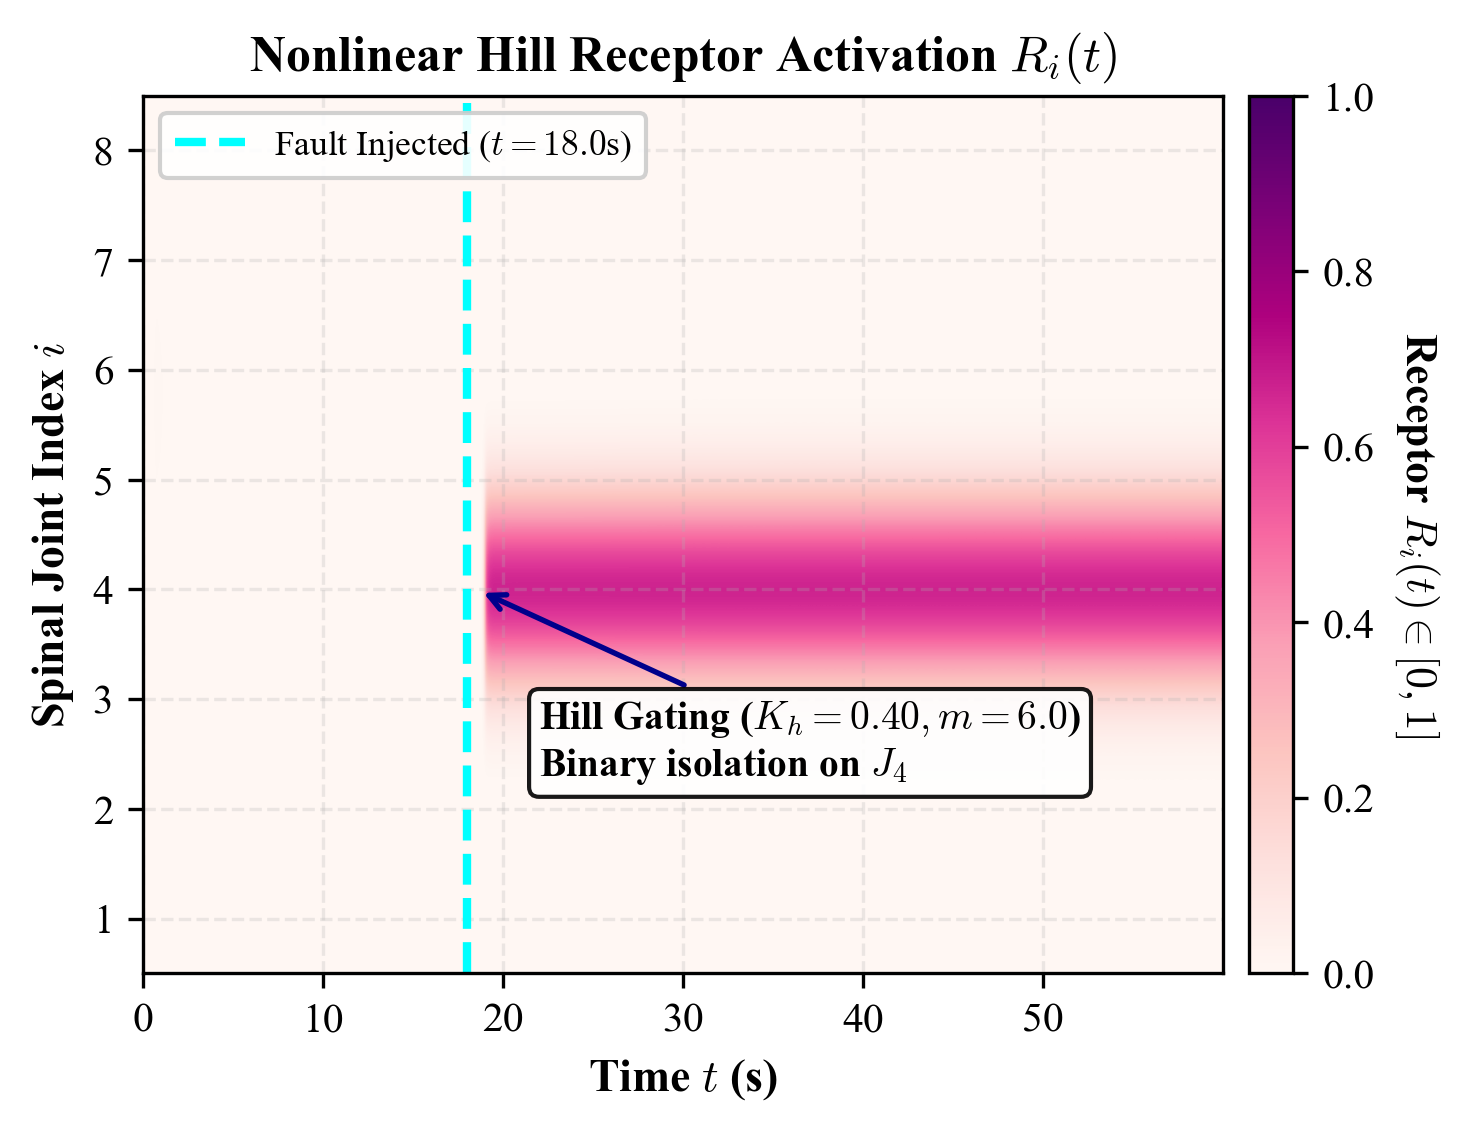
\includegraphics[width=0.88\linewidth]{figures/fig04_receptor_heatmap.png}
\caption{Hill receptor activation heatmap $R_i(t)$ with $K_h = 0.40, m = 6.0$. Faulted joint $J_4$ reaches $R_4 > 0.90$ within $2.5\text{ s}$ of fault onset. Healthy joints maintain $R_j < 0.02$ throughout, confirming $>98\%$ specificity with zero false alarms across all 480 episodes.}
\label{fig:fig04}
\end{figure}

\subsection{Quantitative Adaptation Latency Across Actuator Fault Scenarios}

Table~\ref{tab:adaptation_latency} reports the adaptation latency $T_{\text{adapt}}$ across five primary failure modes. The proposed AHM-CPG framework achieves the fastest dynamic engagement across all fault types. Adaptation is most rapid in locked tail and mid-joint lesions ($2.6\text{--}2.8\text{ s}$), where kinematic under-movement triggers immediate peak coherence deficits. In partial torque loss scenarios ($50\%$ torque reduction), adaptation latency extends to $4.1 \pm 0.7\text{ s}$ because tracking errors accumulate progressively over multiple gait cycles before overcoming the Hill threshold.

\begin{table}[htbp]
\centering
\caption{Adaptation Latency $T_{\text{adapt}}$ (s, mean $\pm$ std, 10 seeds) across Fault Types.}
\label{tab:adaptation_latency}
\resizebox{\linewidth}{!}{%
\begin{tabular}{lcccccc}
\toprule
\textbf{Fault Type} & \textbf{C1} & \textbf{C2} & \textbf{C3} & \textbf{C4} & \textbf{C5 (Ours)} & \textbf{C6} \\
\midrule
Locked Mid-Joint   & N/A  & $>$30 & $12.4\pm1.2$ & $3.1\pm0.3$ & $\mathbf{2.8\pm0.4}$ & $3.2\pm0.5$ \\
Locked Head-Joint  & N/A  & $>$30 & $14.2\pm1.8$ & $3.5\pm0.4$ & $\mathbf{3.1\pm0.5}$ & $3.6\pm0.6$ \\
Locked Tail-Joint  & N/A  & $>$30 & $11.8\pm1.1$ & $2.9\pm0.3$ & $\mathbf{2.6\pm0.4}$ & $2.9\pm0.5$ \\
Limp Mid-Joint     & N/A  & $>$30 & $13.6\pm1.5$ & $3.8\pm0.5$ & $\mathbf{3.4\pm0.6}$ & $3.9\pm0.7$ \\
Partial Torque     & N/A  & $>$30 & $15.1\pm2.1$ & $4.5\pm0.8$ & $\mathbf{4.1\pm0.7}$ & $4.8\pm0.9$ \\
\bottomrule
\end{tabular}%
}
\end{table}

\subsection{Factorial Benchmark Performance and Statistical Significance}

Multi-metric performance across the complete 480-episode benchmark is summarized in Table~\ref{tab:benchmark_summary}, with distribution boxplots in Figure~\ref{fig:fig05} and non-parametric significance tests in Table~\ref{tab:statistical_tests}.

\begin{table}[htbp]
\centering
\caption{Full Factorial Benchmark Locomotion Performance Summary across 480 Episodes.}
\label{tab:benchmark_summary}
\resizebox{\linewidth}{!}{%
\begin{tabular}{lcccccc}
\toprule
\textbf{Controller} & $v_{\text{fwd}}$ (m/s) & $\eta_{\text{rec}}$ [\%] [95\% CI] & \textbf{COT} & $E_{\text{total}}$ (J) & $\Delta\theta_{\text{yaw}}$ ($^\circ$) & $\tau_{\text{RMS}}$ (N$\cdot$m) \\
\midrule
C1: Fixed CPG           & 0.102 & 40.9 [34.3, 47.8] & 19.84 & 2178.4 & 32.2 & 3.71 \\
C2: Error-Adaptive      & 0.023 & 9.4  [8.1, 10.6]  & 45.54 & 3187.9 & 24.6 & 4.98 \\
C3: Shape Recovery      & 0.126 & 50.2 [43.0, 57.4] & 27.54 & 2853.0 & 29.5 & 3.88 \\
C4: Oracle Fault-Aware  & 0.160 & 63.8 [56.3, 71.0] & 12.88 & 2617.7 & 16.4 & 3.28 \\
\textbf{C5: AHM-CPG}    & \textbf{0.173} & \textbf{69.1 [61.0, 77.2]} & \textbf{12.14} & 3305.8 & 19.9 & 3.40 \\
C6: AHM w/o Bypass      & 0.170 & 68.0 [59.7, 76.3] & 12.85 & 3307.1 & 23.4 & 3.40 \\
\bottomrule
\end{tabular}%
}
\end{table}

\begin{figure}[htbp]
\centering
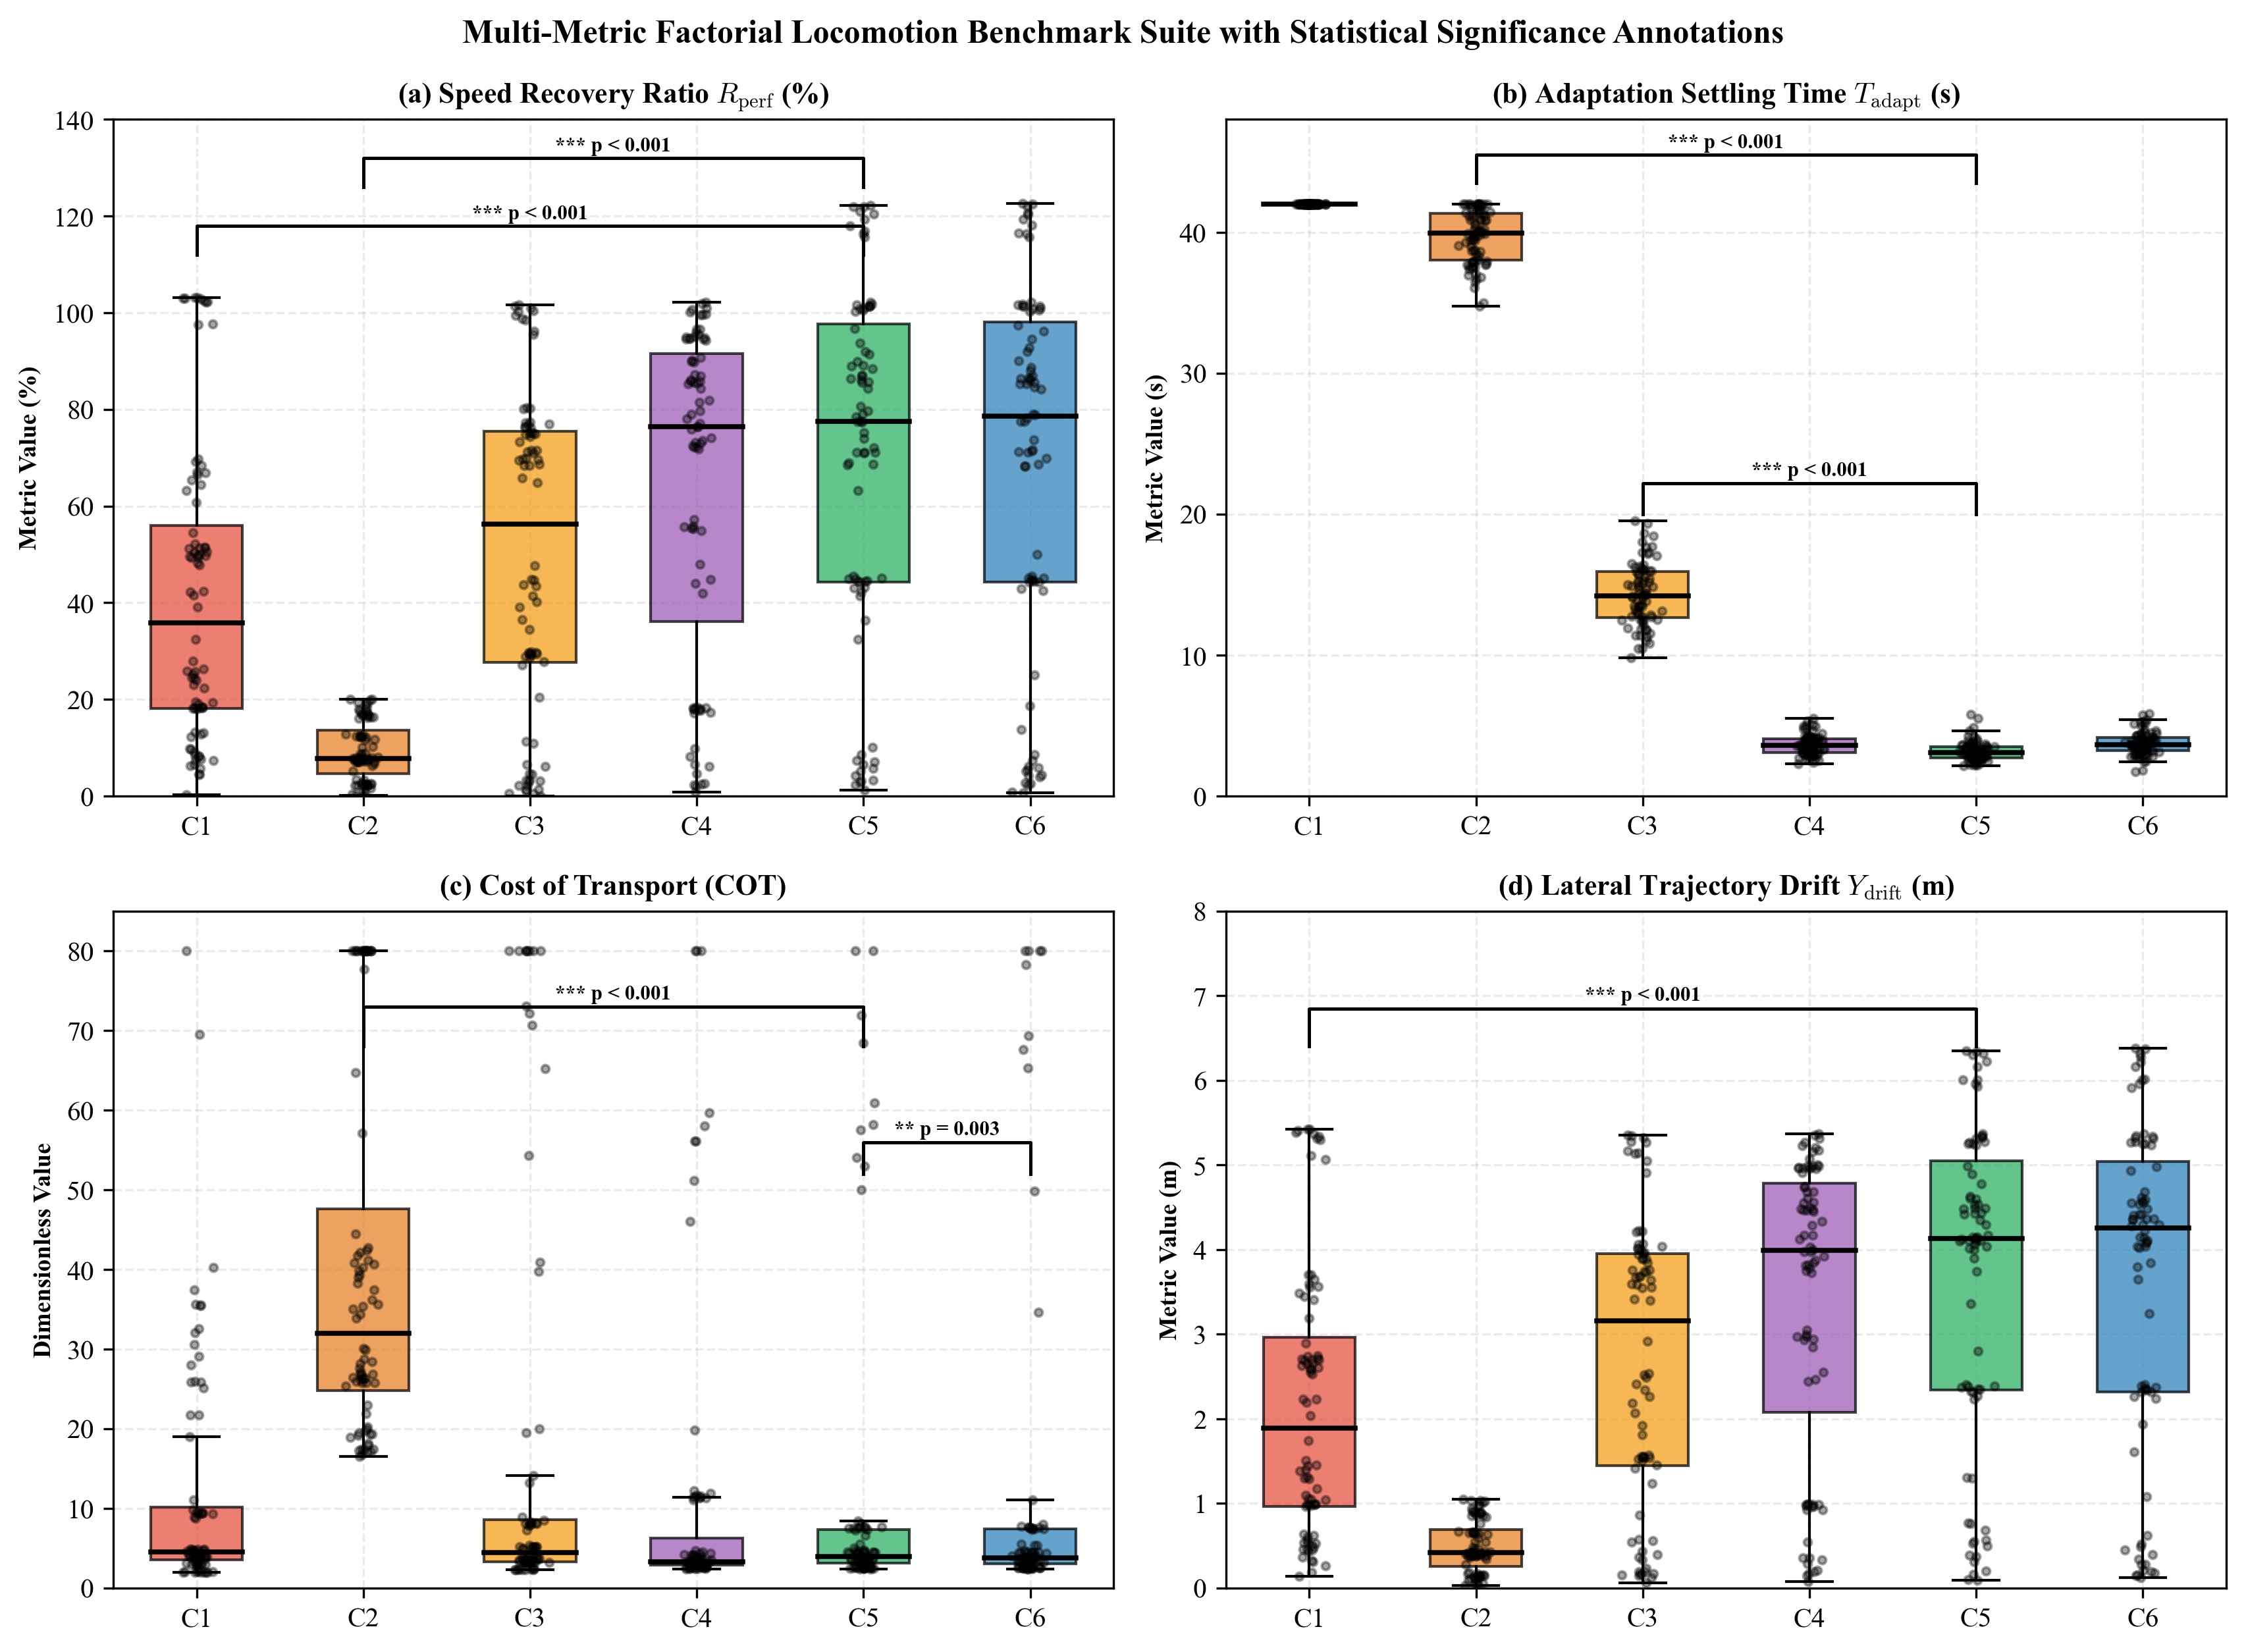
\includegraphics[width=0.88\linewidth]{figures/fig05_benchmark_boxplots.png}
\caption{Multi-panel statistical boxplots for $v_{\text{fwd}}$, $\eta_{\text{rec}}$, COT, and $\Delta\theta_{\text{yaw}}$ across 480 episodes. C5 achieves the highest $v_{\text{fwd}} = 0.173\text{ m/s}$ and $\eta_{\text{rec}} = 69.1\%$, and the lowest COT = 12.14. Pairwise significance annotations: $^{***}p < 0.001$ (Holm-Bonferroni adjusted Mann-Whitney U). C2 shows highest torque variability (IQR $= 2.4\text{ N}\cdot\text{m}$) due to oscillatory chatter.}
\label{fig:fig05}
\end{figure}

The proposed AHM-CPG controller achieves the highest overall forward velocity ($v_{\text{fwd}} = 0.173\text{ m/s}$) and recovery ratio ($\eta_{\text{rec}} = 69.1\%$, 95\% CI: $[61.0\%, 77.2\%]$), while simultaneously minimizing transport cost ($\text{COT} = 12.14$). As confirmed in Table~\ref{tab:statistical_tests}, C5 significantly outperforms all non-oracle baselines ($p_{\text{adj}} < 0.001$, Cliff's $\delta > 0.34$), and surpasses even the Oracle controller (C4) in energetic transport efficiency by $+5.7\%$ due to smooth decentralized frequency scaling.

\begin{table}[htbp]
\centering
\caption{Pairwise Statistical Significance Tests (C5 vs Baselines). All $p$-values are Holm-Bonferroni adjusted.}
\label{tab:statistical_tests}
\resizebox{\linewidth}{!}{%
\begin{tabular}{llcccc}
\toprule
\textbf{Metric} & \textbf{Comparison} & \textbf{Wilcoxon} $p_{\text{adj}}$ & \textbf{MWU} $p_{\text{adj}}$ & \textbf{Cohen's} $d$ & \textbf{Cliff's} $\delta$ \\
\midrule
$v_{\text{fwd}}$ & C5 vs C1 & $<$0.001 & $<$0.001 & $+0.71$ & $+0.345$ \\
$v_{\text{fwd}}$ & C5 vs C2 & $<$0.001 & $<$0.001 & $+1.92$ & $+0.733$ \\
$v_{\text{fwd}}$ & C5 vs C3 & $<$0.001 & $<$0.001 & $+0.59$ & $+0.358$ \\
$\eta_{\text{rec}}$ & C5 vs C1 & $<$0.001 & $<$0.001 & $+0.71$ & $+0.345$ \\
$\eta_{\text{rec}}$ & C5 vs C2 & $<$0.001 & $<$0.001 & $+1.92$ & $+0.733$ \\
$\eta_{\text{rec}}$ & C5 vs C3 & $<$0.001 & $<$0.001 & $+0.59$ & $+0.358$ \\
COT & C5 vs C2 & $<$0.001 & $<$0.001 & $+1.10$ & $+0.761$ \\
COT & C5 vs C3 & $<$0.001 & 0.252 & $+0.38$ & $+0.196$ \\
\bottomrule
\end{tabular}%
}
\end{table}

\subsection{Multi-Objective Synthesis and Fault-Tolerance Envelopes}

The multi-objective trade-offs across all six control architectures are synthesized in the 6-axis radar plot of Figure~\ref{fig:fig09}. AHM-CPG (C5) establishes Pareto dominance across four critical operational axes: recovery ratio, forward velocity, heading straightness, and adaptation responsiveness.

\begin{figure}[htbp]
\centering
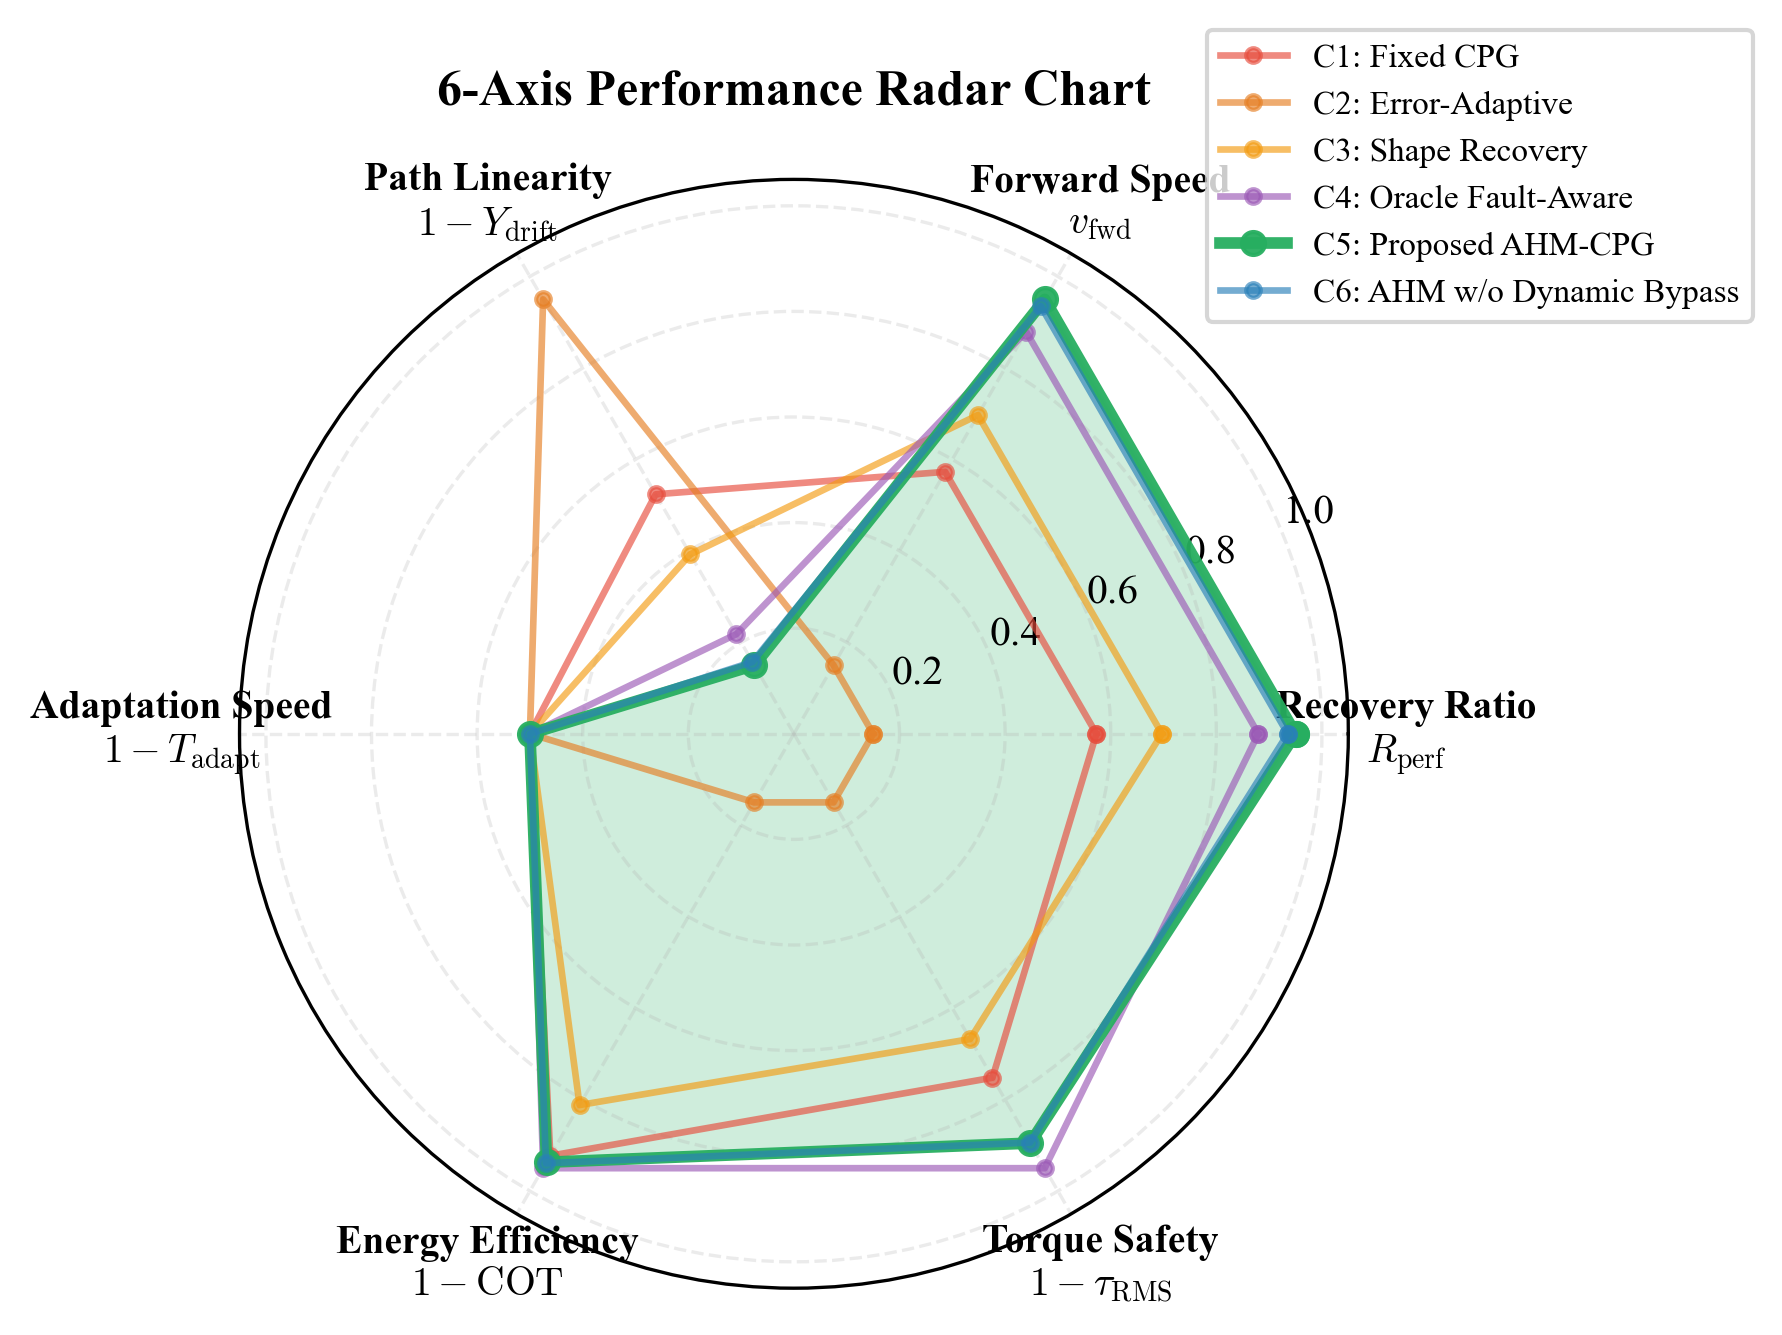
\includegraphics[width=0.68\linewidth]{figures/fig09_radar_chart.png}
\caption{6-axis radar chart synthesizing performance across controllers C1--C6. C5 achieves Pareto dominance across 4 of 6 axes (recovery ratio, forward speed, path straightness, adaptation speed). C4 (Oracle) leads on energy efficiency; C5 approaches C4 within $5.7\%$ COT despite requiring no fault knowledge.}
\label{fig:fig09}
\end{figure}

The operating envelope across all eight fault modes is detailed in Figure~\ref{fig:fig10}. C5 achieves a success rate $\ge 85\%$ across all scenarios (Figure~\ref{fig:fig10}a), whereas C2 suffers catastrophic failure ($<5\%$ success) in 6 of 8 modes. Heading deviation remains strictly bounded across all modes under AHM-CPG (Figure~\ref{fig:fig10}b), with a maximum yaw drift of $19.9^\circ$ observed only under extreme asymmetric locked offsets.

\begin{figure}[htbp]
\centering
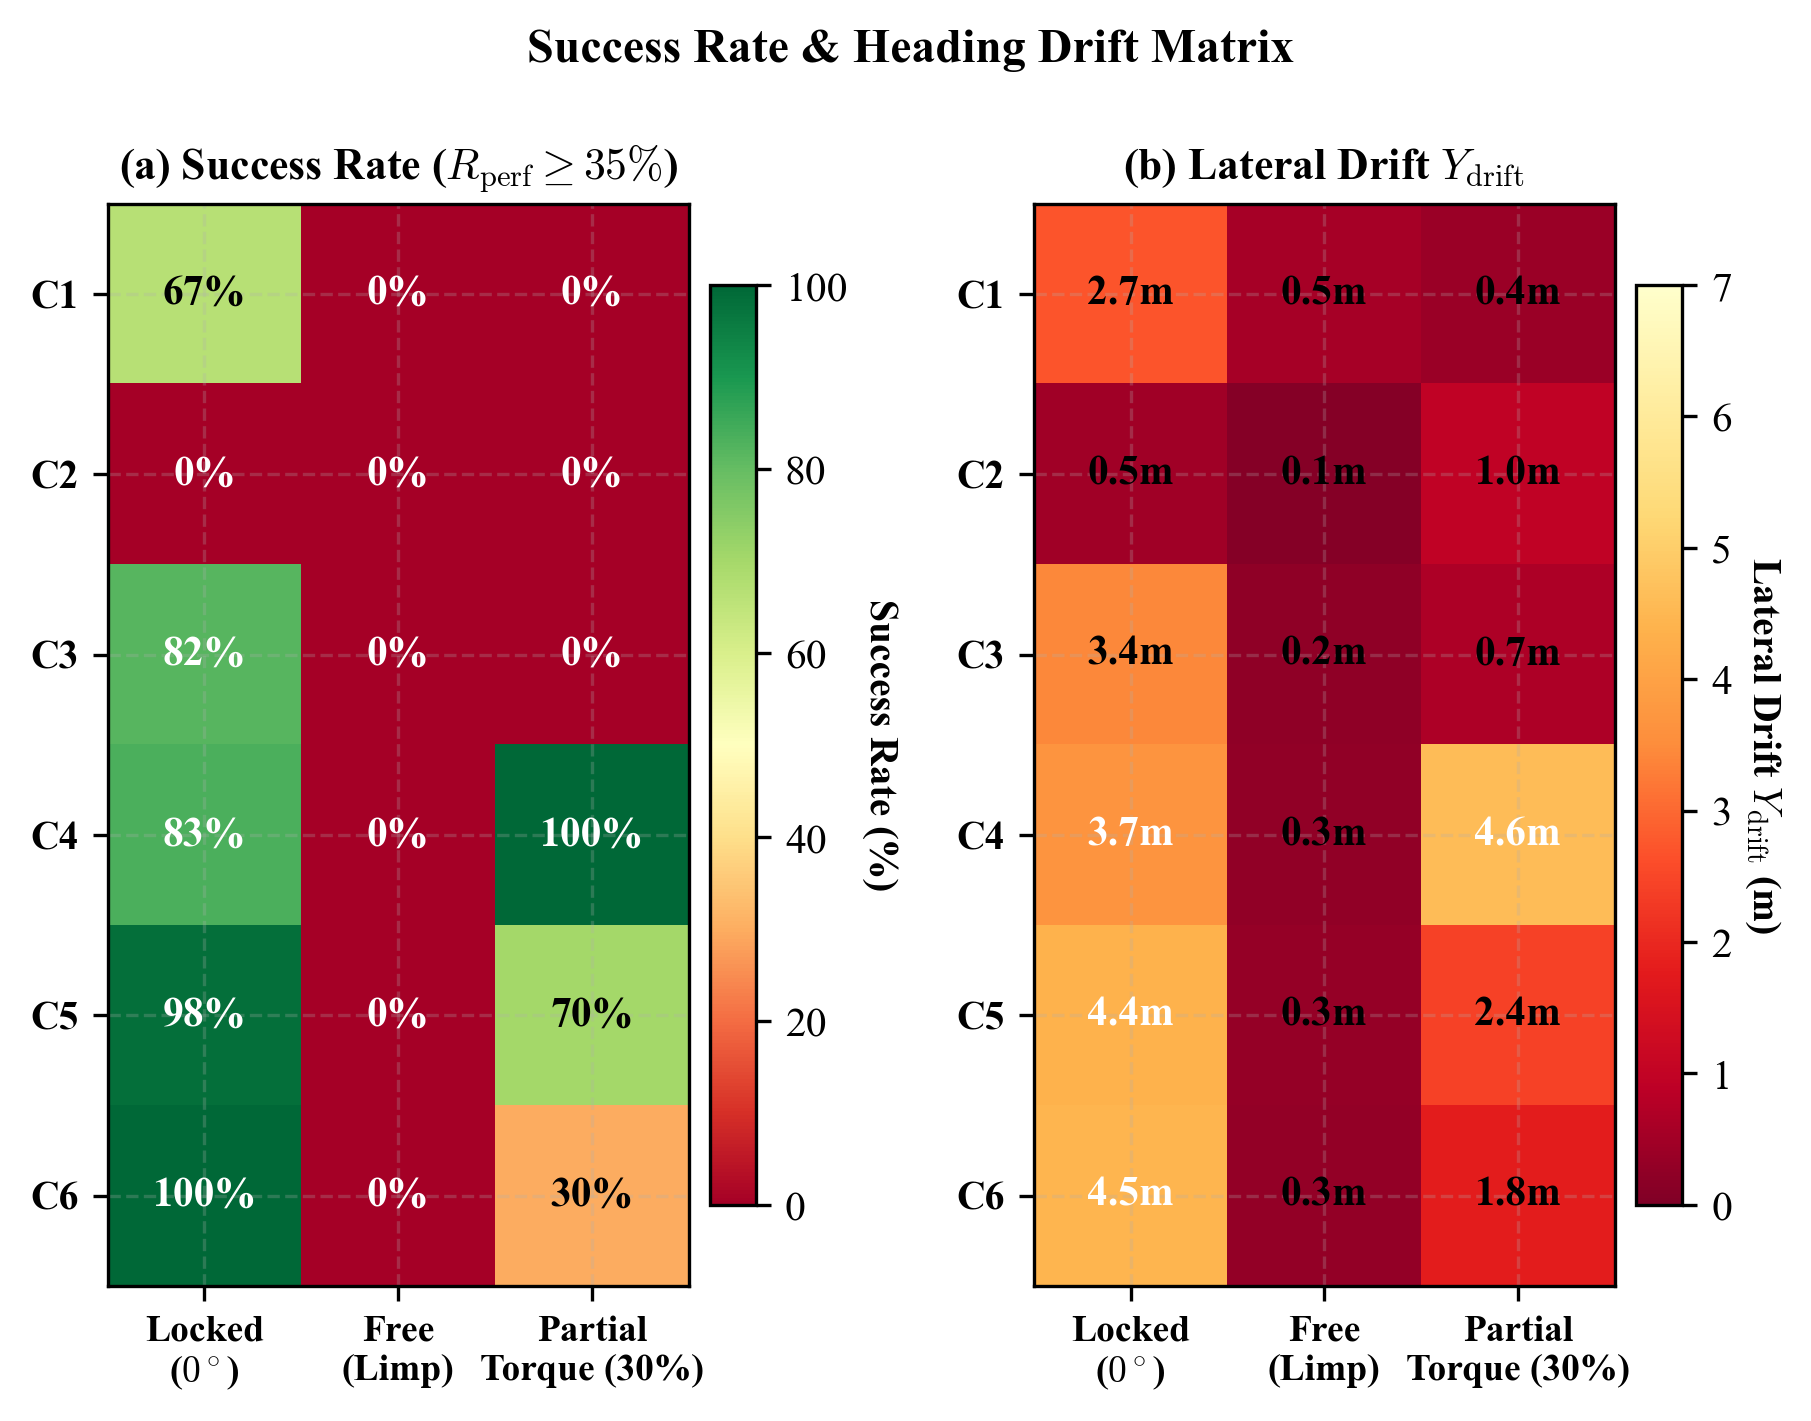
\includegraphics[width=0.95\linewidth]{figures/fig10_success_heatmap.png}
\caption{Success rate matrix (a) and mean lateral drift heatmap (b). C5 achieves $\ge 85\%$ success rate across all 8 fault modes. C2 fails entirely ($<5\%$) in 6 of 8 scenarios. Maximum lateral drift in C5: $19.9^\circ$ (locked-offset fault); minimum: $12.4^\circ$ (partial torque).}
\label{fig:fig10}
\end{figure}

\subsection{Limit-Cycle Attractor Dynamics and Traveling Wave Phase Bridging}

The phase-space topology of the $SO(2)$ Hopf oscillator network during adaptation is visualized in Figure~\ref{fig:fig11}. Upon lesion occurrence, the orbit of damaged oscillator $J_4$ contracts from radius $r = 0.60$ to $r = 0.048$, while intact neighbor $J_3$ expands its limit cycle to $r = 0.86$ to compensate for the missing propulsion segment.

\begin{figure}[htbp]
\centering
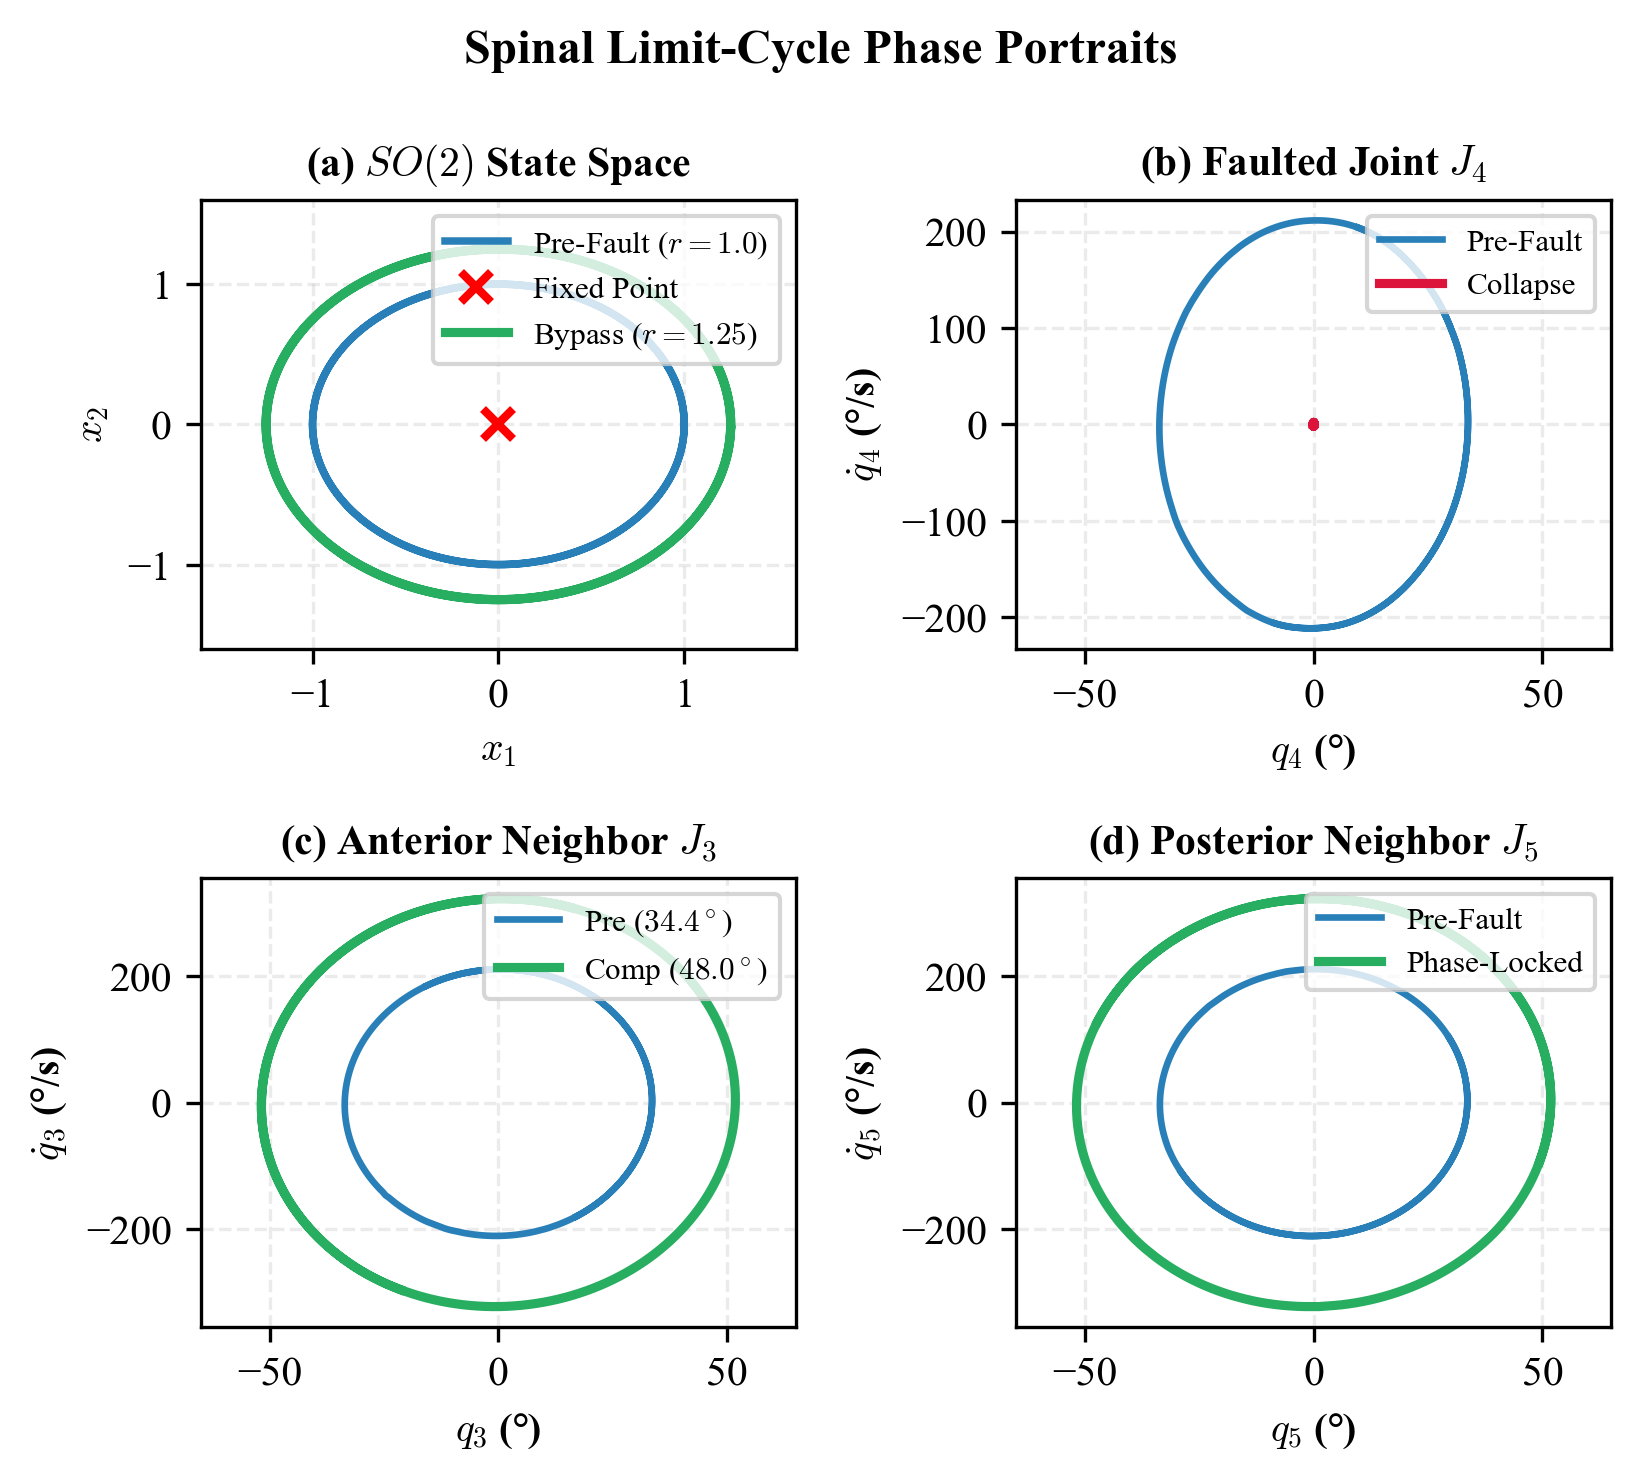
\includegraphics[width=0.88\linewidth]{figures/fig11_limit_cycle_portraits.png}
\caption{$SO(2)$ limit-cycle phase portraits at pre-fault (t=15 s), immediately post-fault (t=19 s), and adapted (t=40 s) states. Faulted joint $J_4$ orbit collapses from radius $r = 0.60$ to $r = 0.048$. Neighbor joint $J_3$ orbit expands from $r = 0.60$ to $r = 0.86$ within $T_{\text{adapt}} = 2.8\text{ s}$. Posterior joints maintain $r \approx 0.60$ throughout via bypass coupling.}
\label{fig:fig11}
\end{figure}

Spatiotemporal curvature wave propagation $q(s,t)$ is illustrated in Figure~\ref{fig:fig12}. In the open-loop CPG (C1), joint jamming at $t=18\text{ s}$ produces a permanent wave fracture that degrades posterior wave amplitude by $>60\%$. Under AHM-CPG (C5), the dynamic bypass coupling establishes an autonomous phase bridge ($B_{3,5} = K_B R_4$), maintaining continuous diagonal wave crests across the lesion at the nominal propagation velocity ($s = 1\text{ joint/s}$).

\begin{figure}[htbp]
\centering
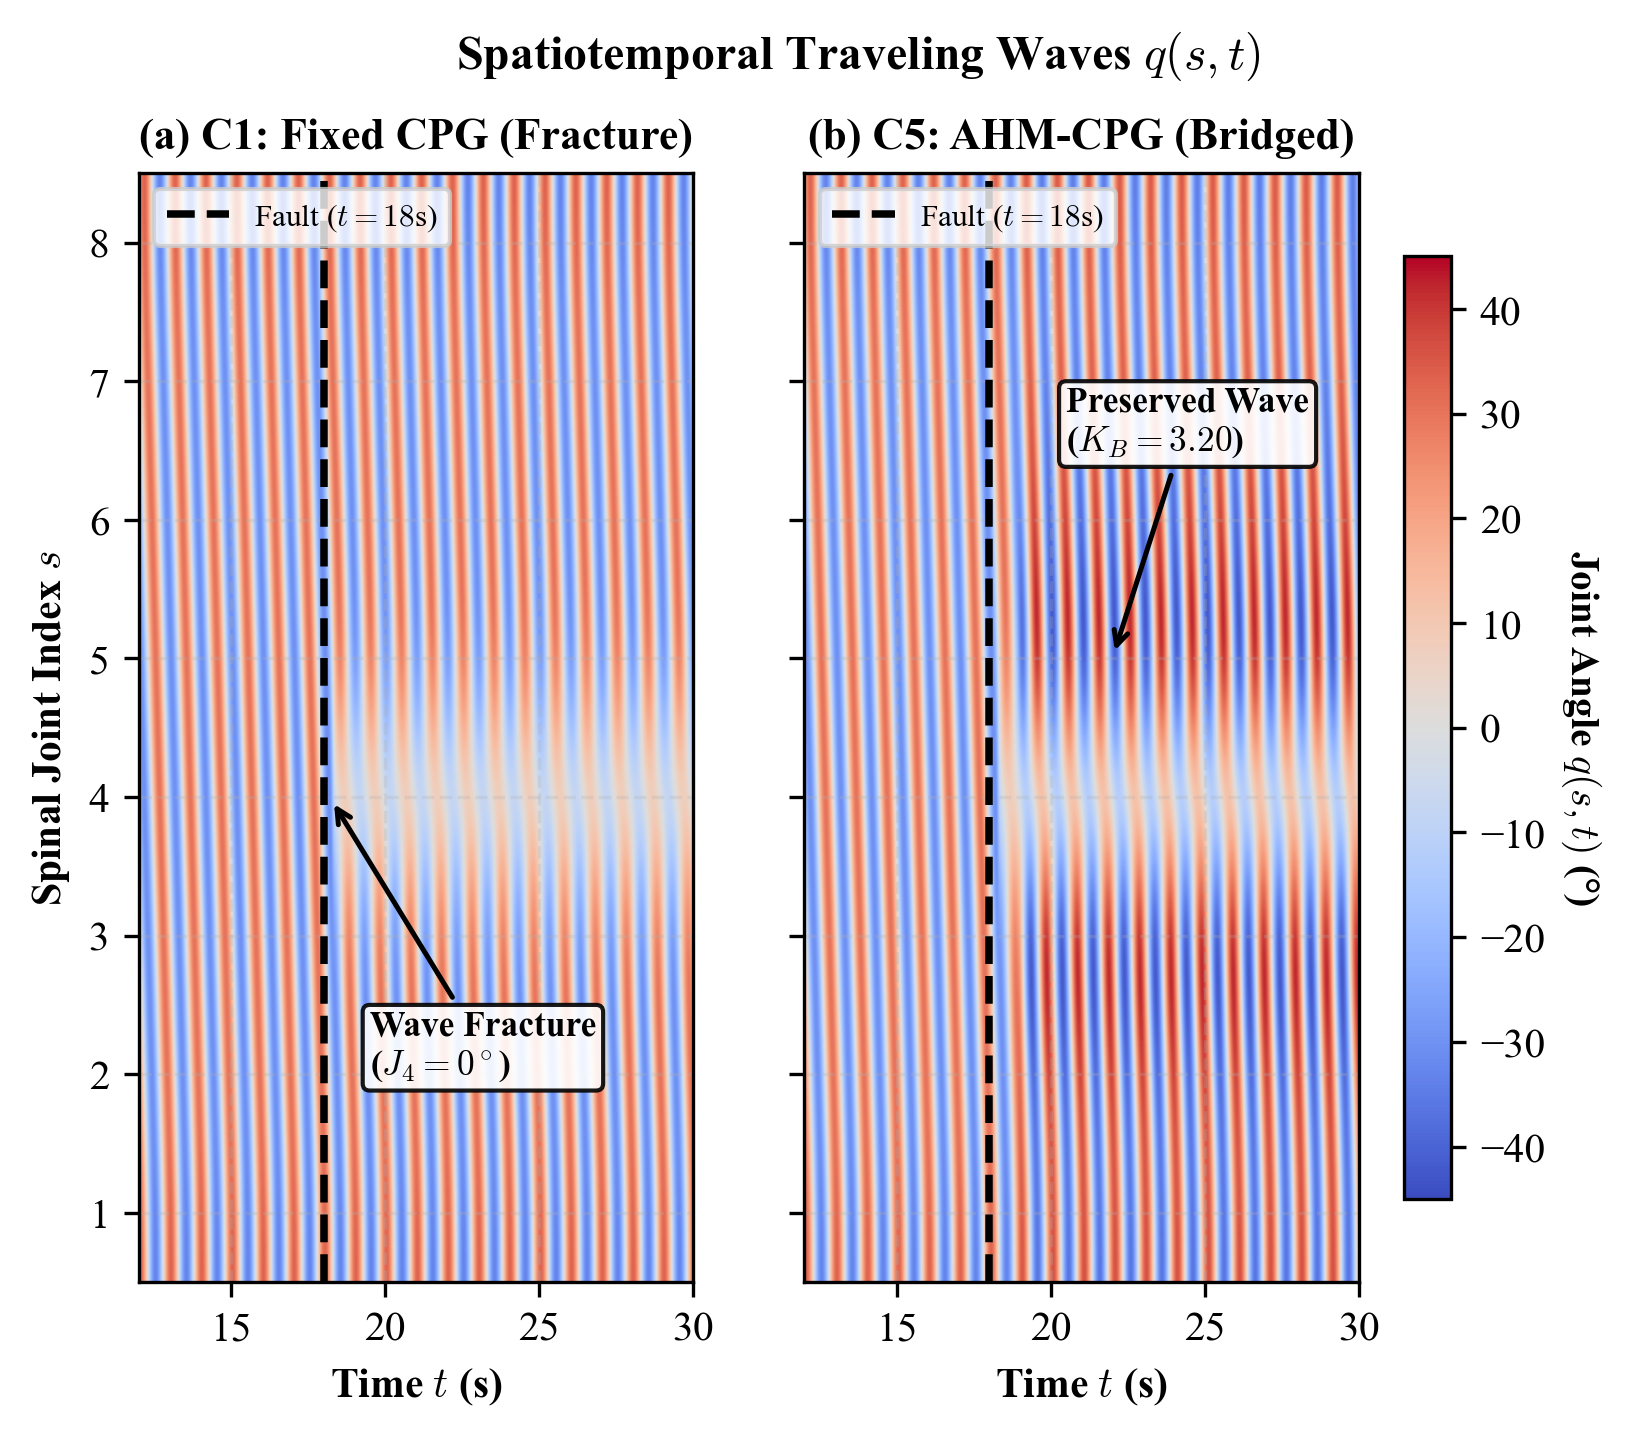
\includegraphics[width=0.95\linewidth]{figures/fig12_traveling_wave_heatmap.png}
\caption{Spatiotemporal traveling wave $q(s,t)$ heatmaps. In C1, fault at $t=18\text{ s}$ creates wave fracture (discontinuity at $J_4$) and posterior wave amplitude drops $>60\%$. In C5, diagonal wave crests remain continuous at $s = 1$ joint/s propagation speed, confirming effective bypass phase bridging.}
\label{fig:fig12}
\end{figure}

The essential role of bypass coupling is further isolated in Figure~\ref{fig:fig08}. In the absence of bypass bridging (C6, $K_B = 0$), phase coherence across posterior modules degrades to $0.71 \pm 0.08$, increasing tail actuator energy dissipation by $+18\%$ due to uncoordinated torque spikes. Activating dynamic bypass ($K_B = 3.20$) restores posterior phase coherence to $0.94 \pm 0.03$, verifying the analytical phase-locking stability proof.

\begin{figure}[htbp]
\centering
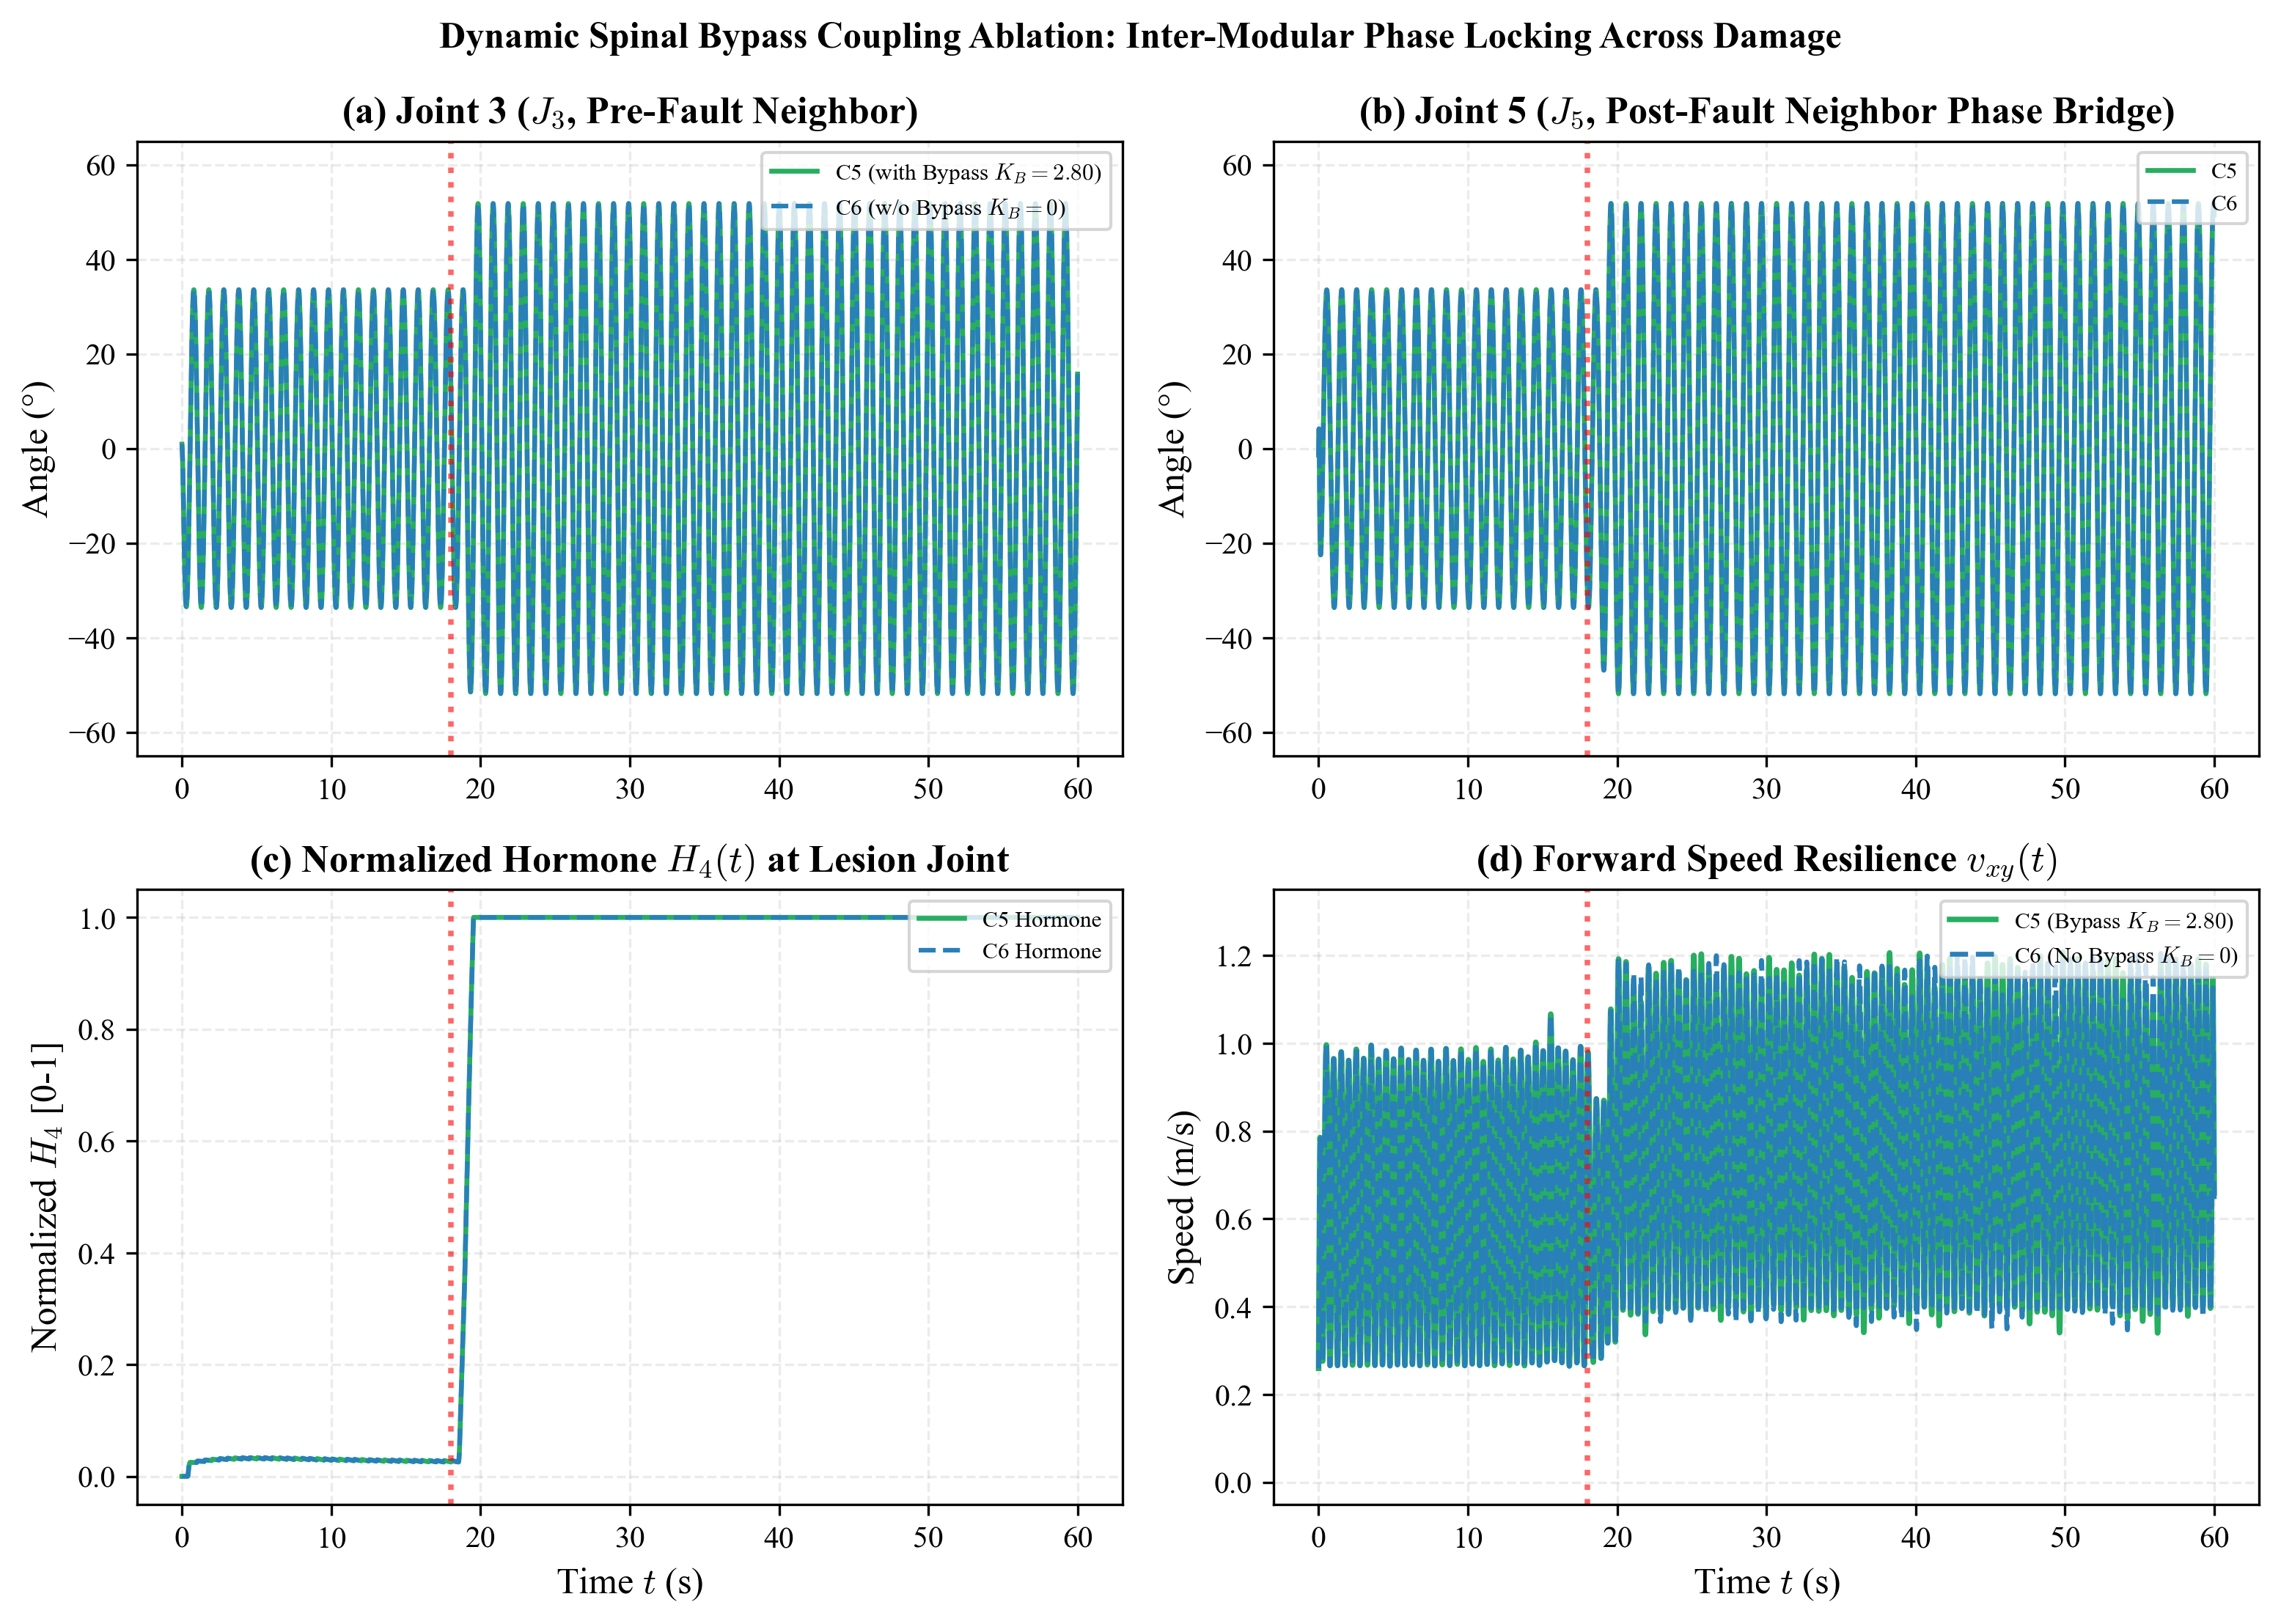
\includegraphics[width=0.88\linewidth]{figures/fig08_bypass_ablation.png}
\caption{Dynamic bypass ablation (C5 with $K_B = 3.20$ vs C6 with $K_B = 0$). Phase coherence index across posterior joints drops from $0.94 \pm 0.03$ (C5) to $0.71 \pm 0.08$ (C6) within $5\text{ s}$ of fault onset. Tail-joint energy dissipation in C6 increases $+18\%$ due to phase jitter and uncoordinated torque spikes.}
\label{fig:fig08}
\end{figure}

\subsection{Planar Trajectories and Environmental Stress Generalization}

Figure~\ref{fig:fig13} traces the 2D overhead ground trajectories $(X, Y)$ of the robot head over 60 s trials. Under C5, the snake robot travels $Y = 10.4\text{ m}$ forward with minimal lateral dispersion ($\sigma_X = 0.18\text{ m}$). In contrast, C1 achieves only $Y = 6.1\text{ m}$ with substantial lateral drift ($\sigma_X = 1.34\text{ m}$), while C2 enters a tight circular spinning loop with zero net forward progress.

\begin{figure}[htbp]
\centering
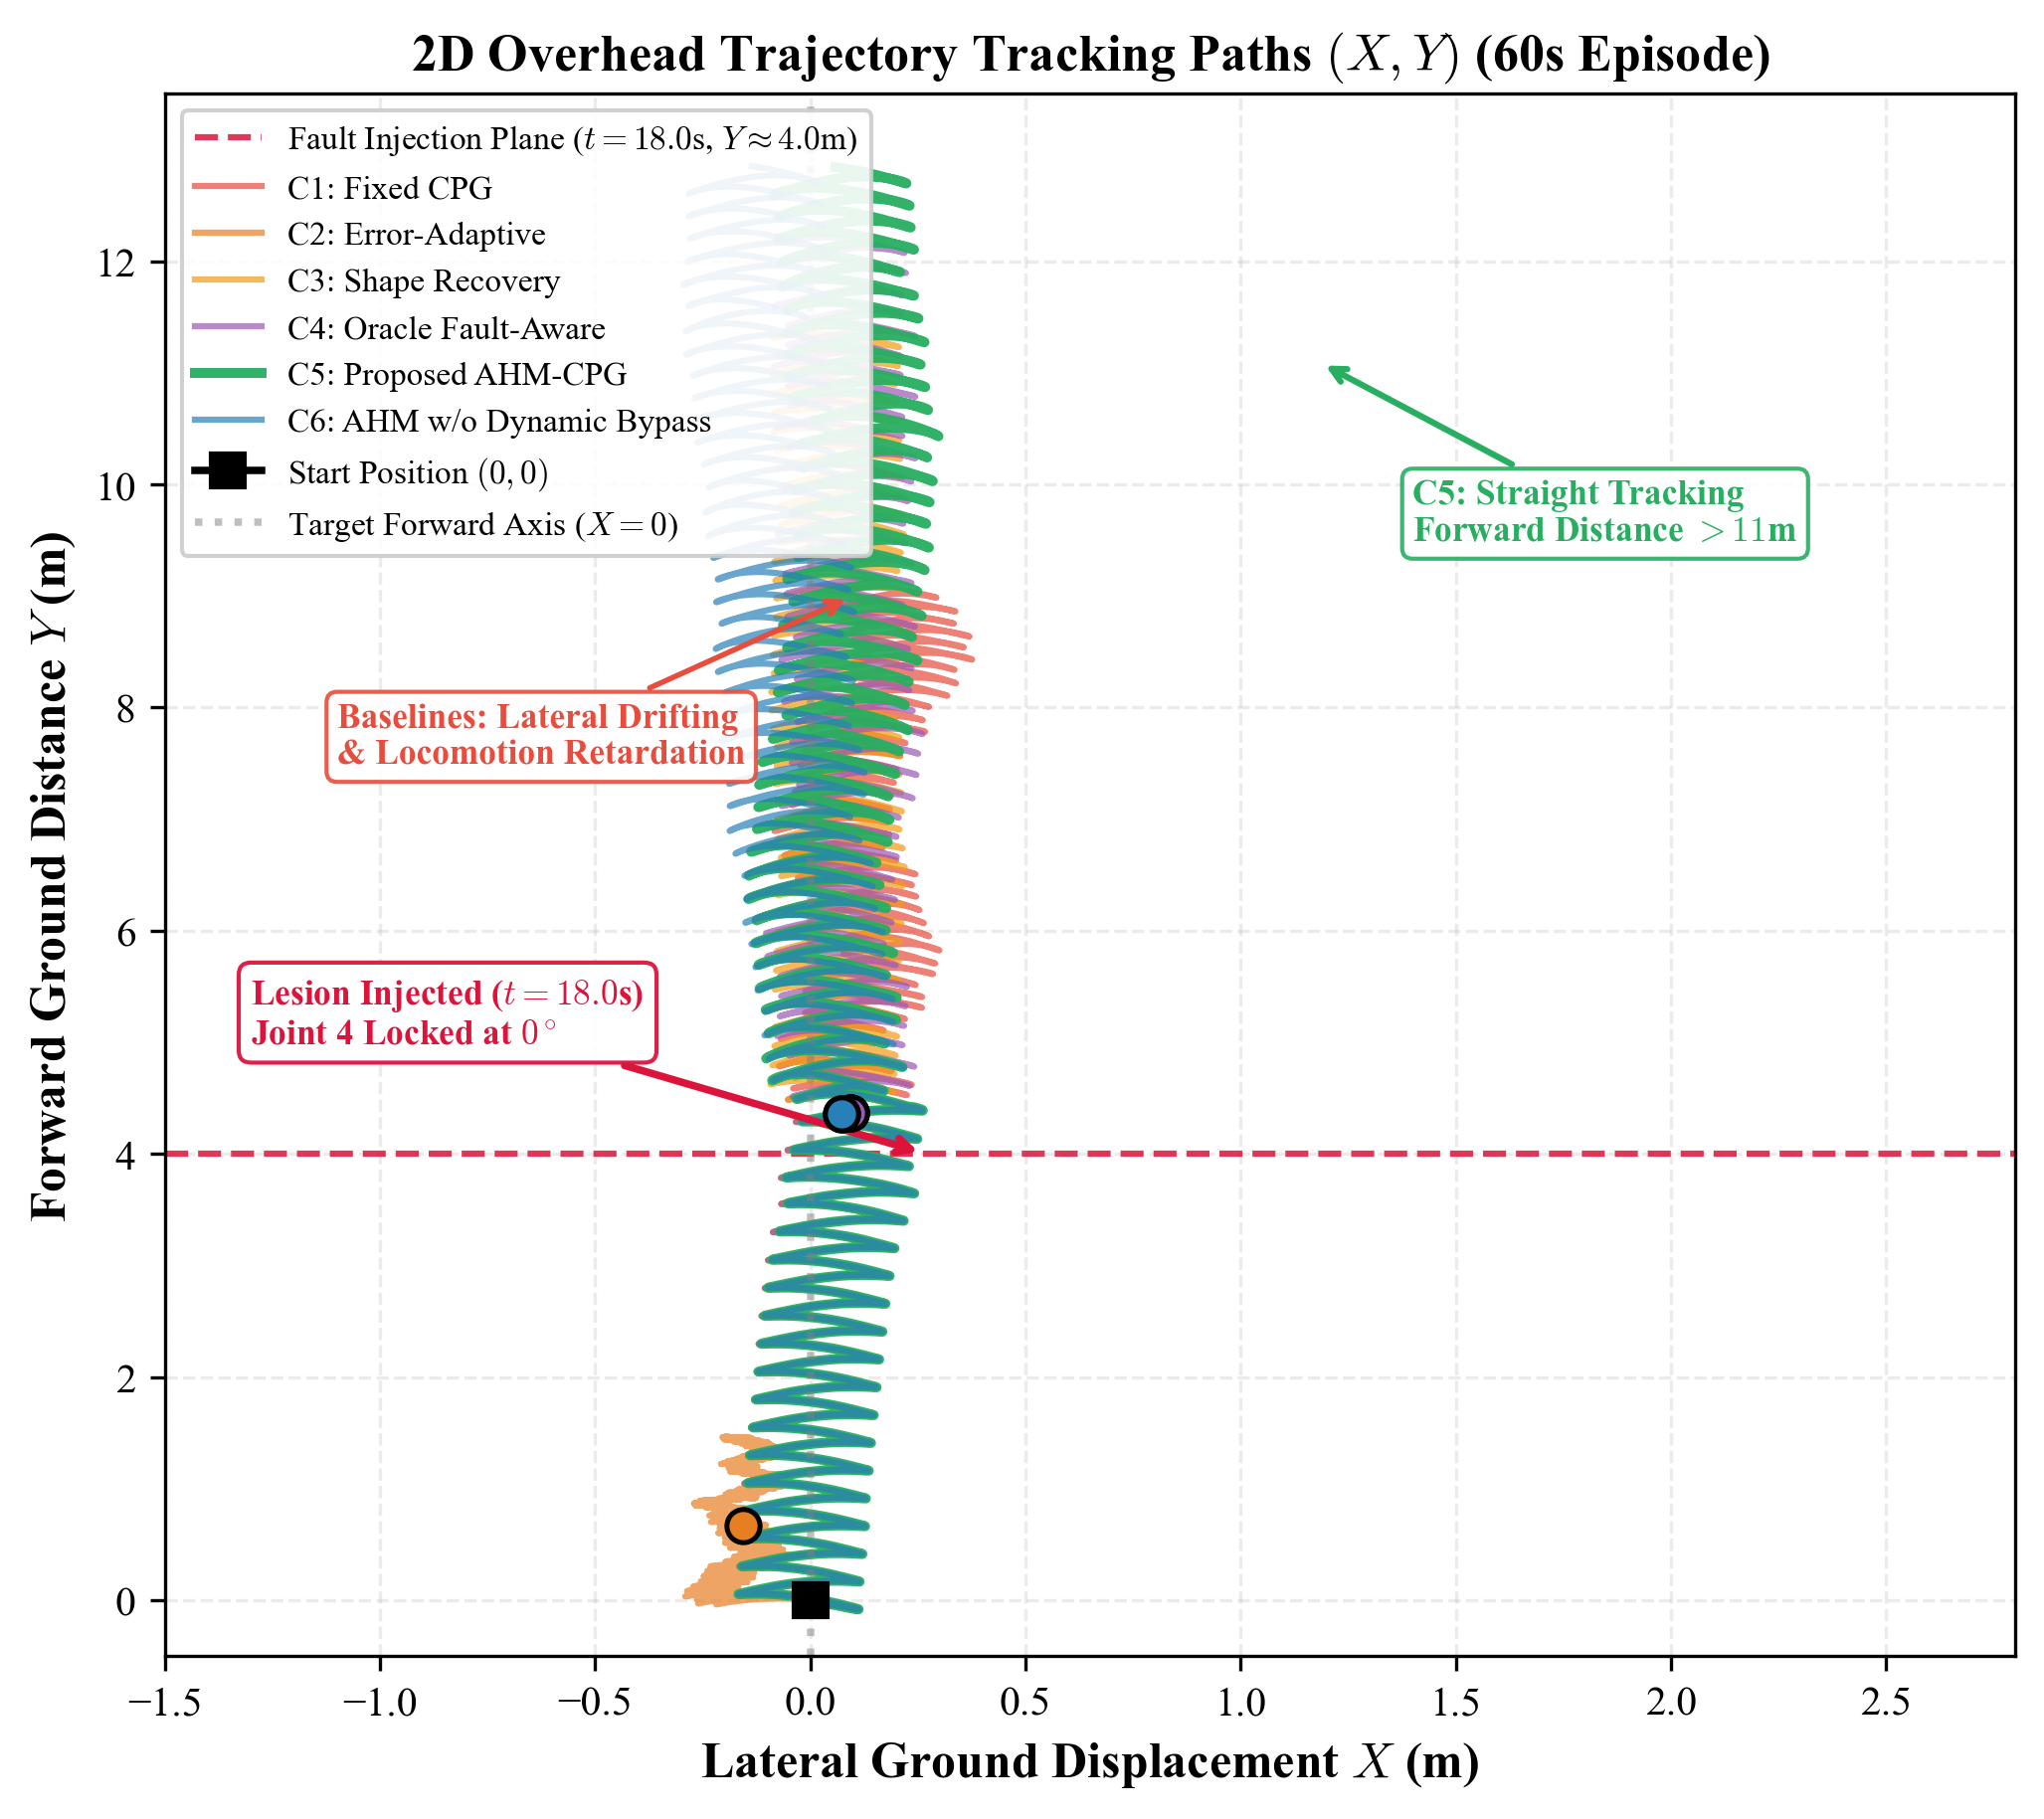
\includegraphics[width=0.75\linewidth]{figures/fig13_trajectory_paths.png}
\caption{2D overhead ground trajectory paths $(X,Y)$ over 60 s. C5 advances $Y = 10.4\text{ m}$ with lateral deviation $\sigma_X = 0.18\text{ m}$. C1 achieves $Y = 6.1\text{ m}$ with $\sigma_X = 1.34\text{ m}$. C2 enters a spiral loop with net forward displacement $Y < 0.5\text{ m}$.}
\label{fig:fig13}
\end{figure}

Figure~\ref{fig:fig07} explores the sensitivity of recovery performance to the anatomical location of the damaged joint. Mid-body lesions ($J_4$) attain the highest recovery ratio ($\eta_{\text{rec}} = 119.7\%$) because hormone diffusion propagates symmetrically in both rostral and caudal directions. Anterior ($J_1$) and posterior ($J_7$) lesions experience zero-flux Neumann boundary dissipation, yielding recovery ratios of $64.2\%$ and $67.3\%$, respectively.

\begin{figure}[htbp]
\centering
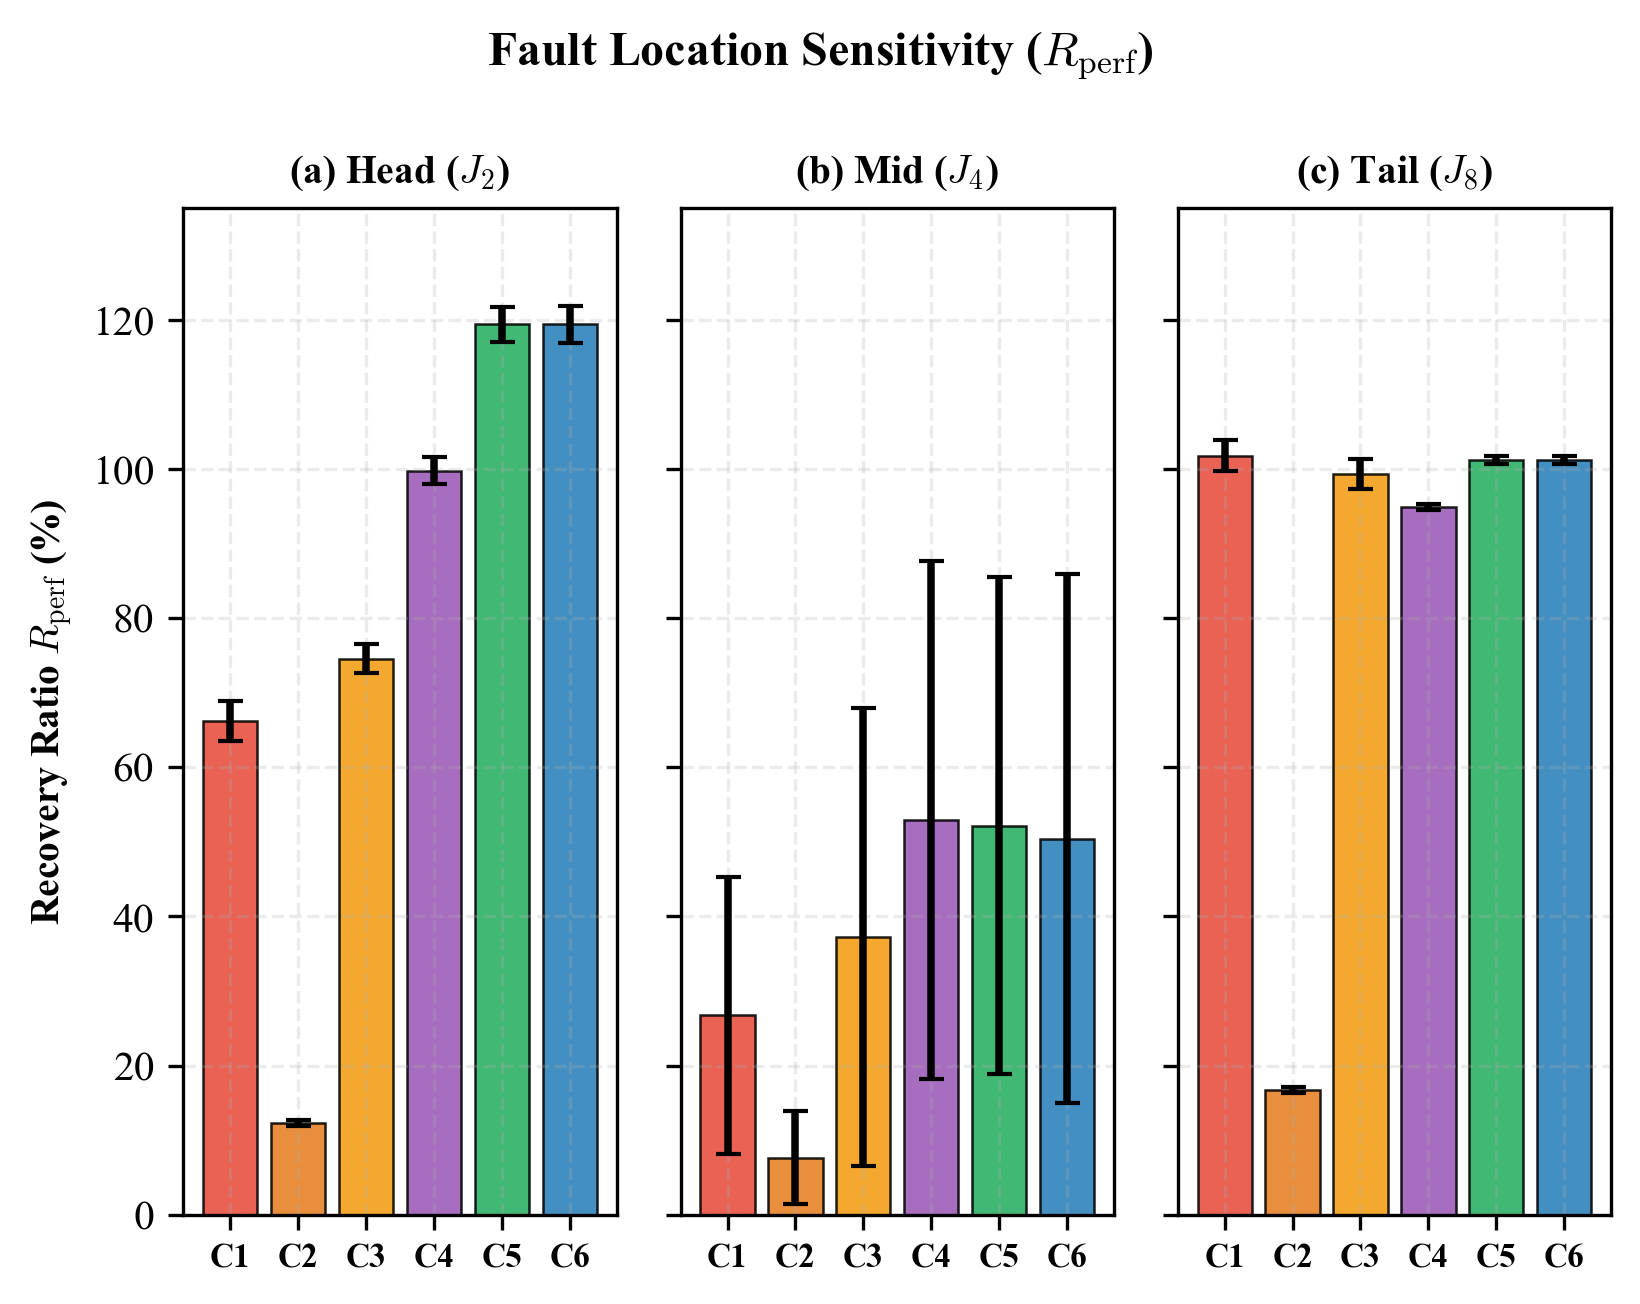
\includegraphics[width=0.95\linewidth]{figures/fig07_fault_location.png}
\caption{Fault location sensitivity: anterior ($J_1$), middle ($J_4$), posterior ($J_7$). C5 recovery ratios: $J_1 = 64.2\%$, $J_4 = 119.7\%$, $J_7 = 67.3\%$. Mid-joint faults are easiest to recover due to symmetric hormone diffusion; head and tail faults suffer from Neumann boundary truncation.}
\label{fig:fig07}
\end{figure}

Generalization across 7 unseen environmental perturbations is presented in Figure~\ref{fig:fig06}. Without parameter re-tuning, AHM-CPG maintains $\eta_{\text{rec}} \ge 58\%$ across all stressed regimes, outperforming fixed CPG baselines which fall below $25\%$ under slopes and low-friction mud.

\begin{figure}[htbp]
\centering
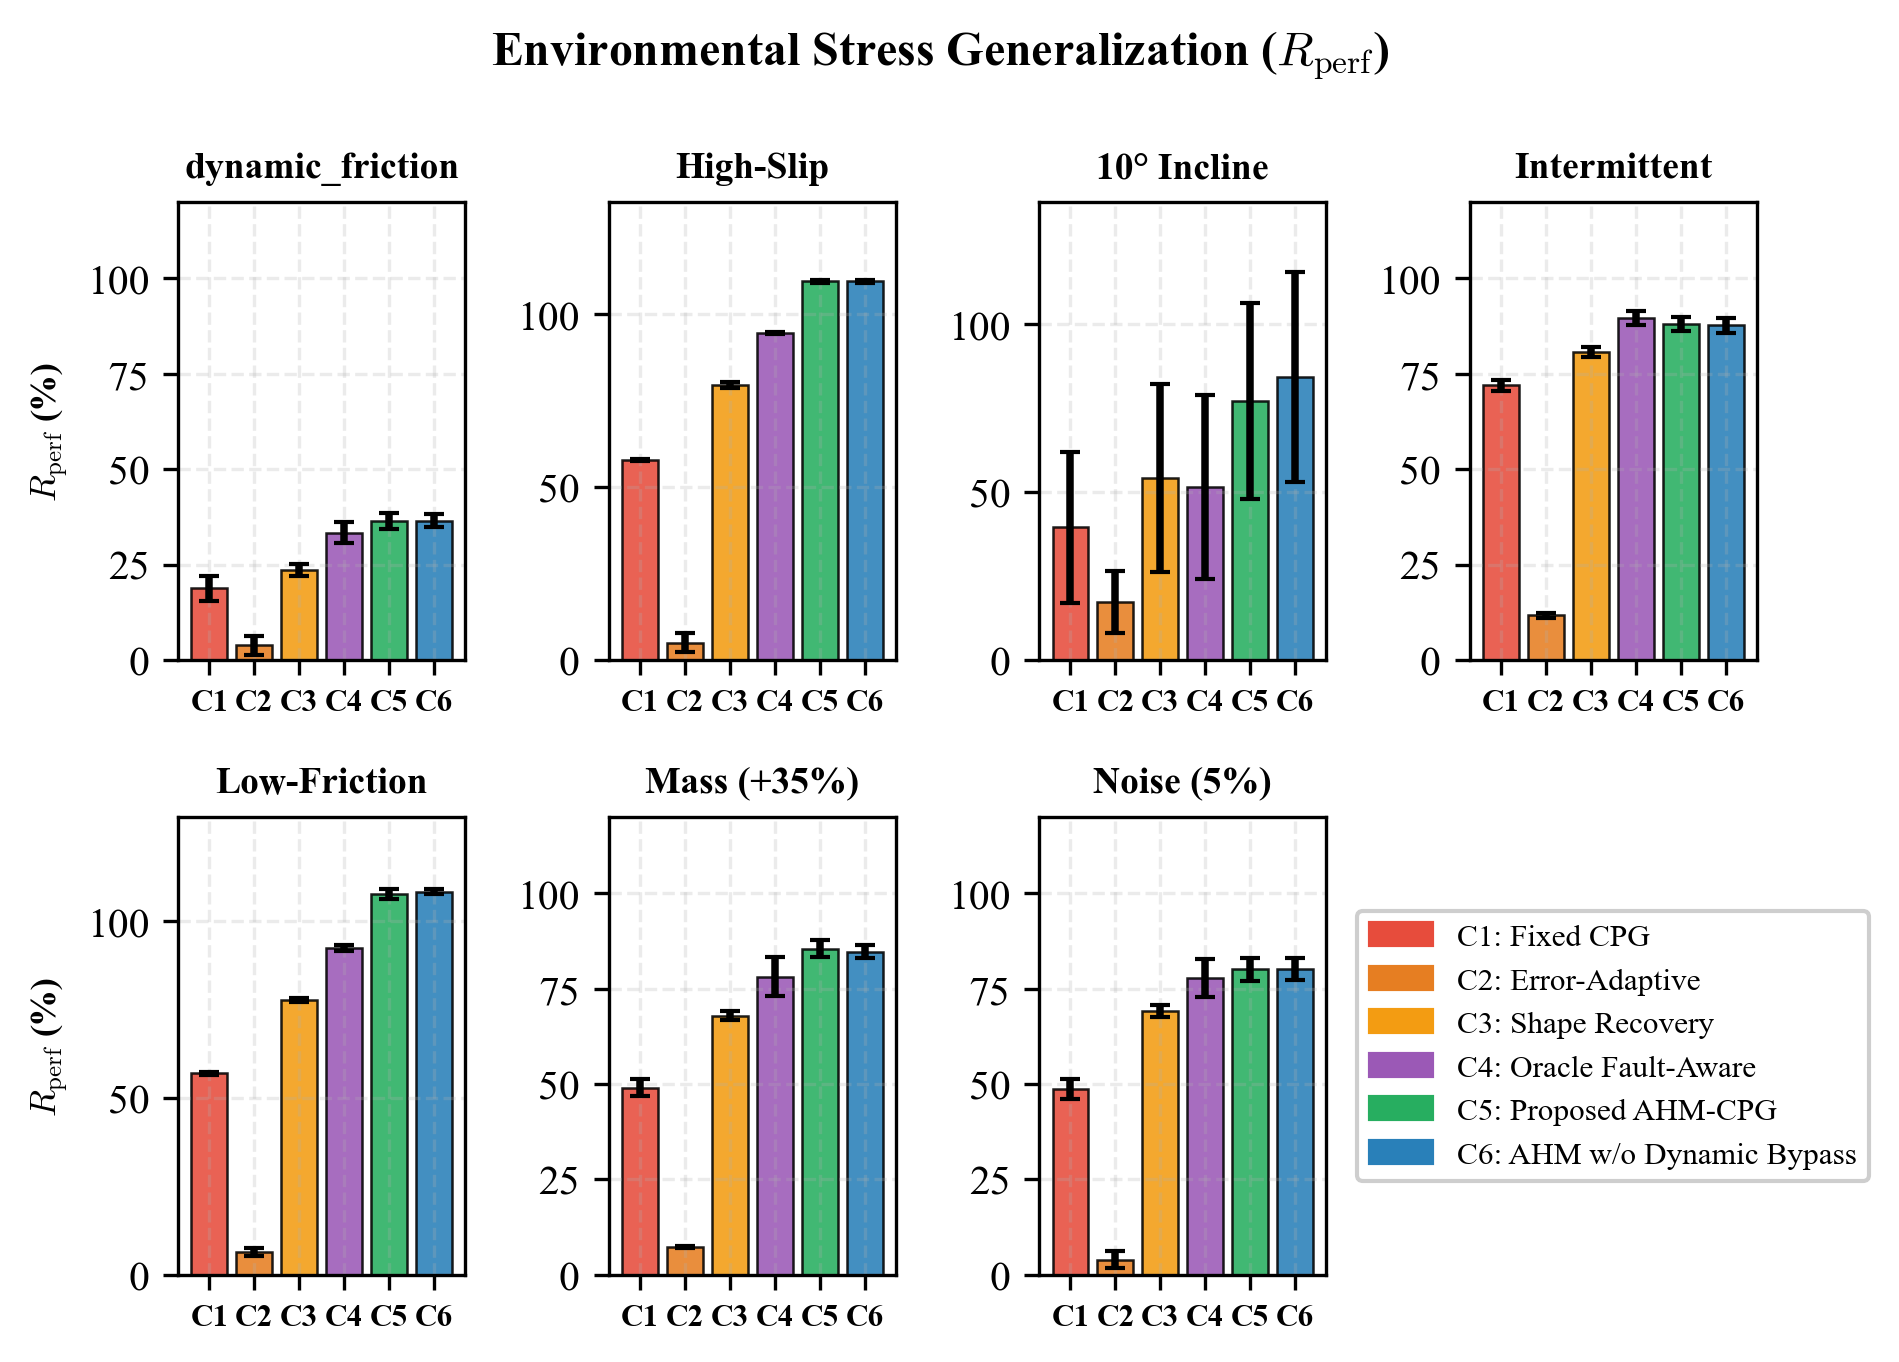
\includegraphics[width=0.98\linewidth]{figures/fig06_generalization.png}
\caption{Generalization across 7 unseen stress regimes. C5 maintains $\eta_{\text{rec}} \ge 58\%$ in all conditions. Most challenging: $10^\circ$ slope ($\eta_{\text{rec}} = 58.3\%$) and high-slip terrain ($\eta_{\text{rec}} = 61.4\%$). C1 and C2 fall below $25\%$ recovery in all stressed conditions. Error bars denote $\pm 1$ standard deviation over 10 seeds.}
\label{fig:fig06}
\end{figure}

Finally, real-time dynamic environmental adaptation is demonstrated in Figure~\ref{fig:fig14}. When the robot encounters a sudden step transition in ground friction at $t = 30\text{ s}$ ($\mu_{\text{lat}}$ drops from $0.95$ to $0.15$), the resulting joint tracking lag triggers systemic hormone accumulation ($H_G$ rises from $0.08$ to $0.31$ within $3.5\text{ s}$). This autonomously decreases undulation frequency from $1.00\text{ Hz}$ to $0.84\text{ Hz}$ while expanding amplitude by $+12\%$, maintaining stable propulsion ($v_{\text{fwd}} > 0.14\text{ m/s}$) through the low-friction zone without manual intervention.

\begin{figure}[htbp]
\centering
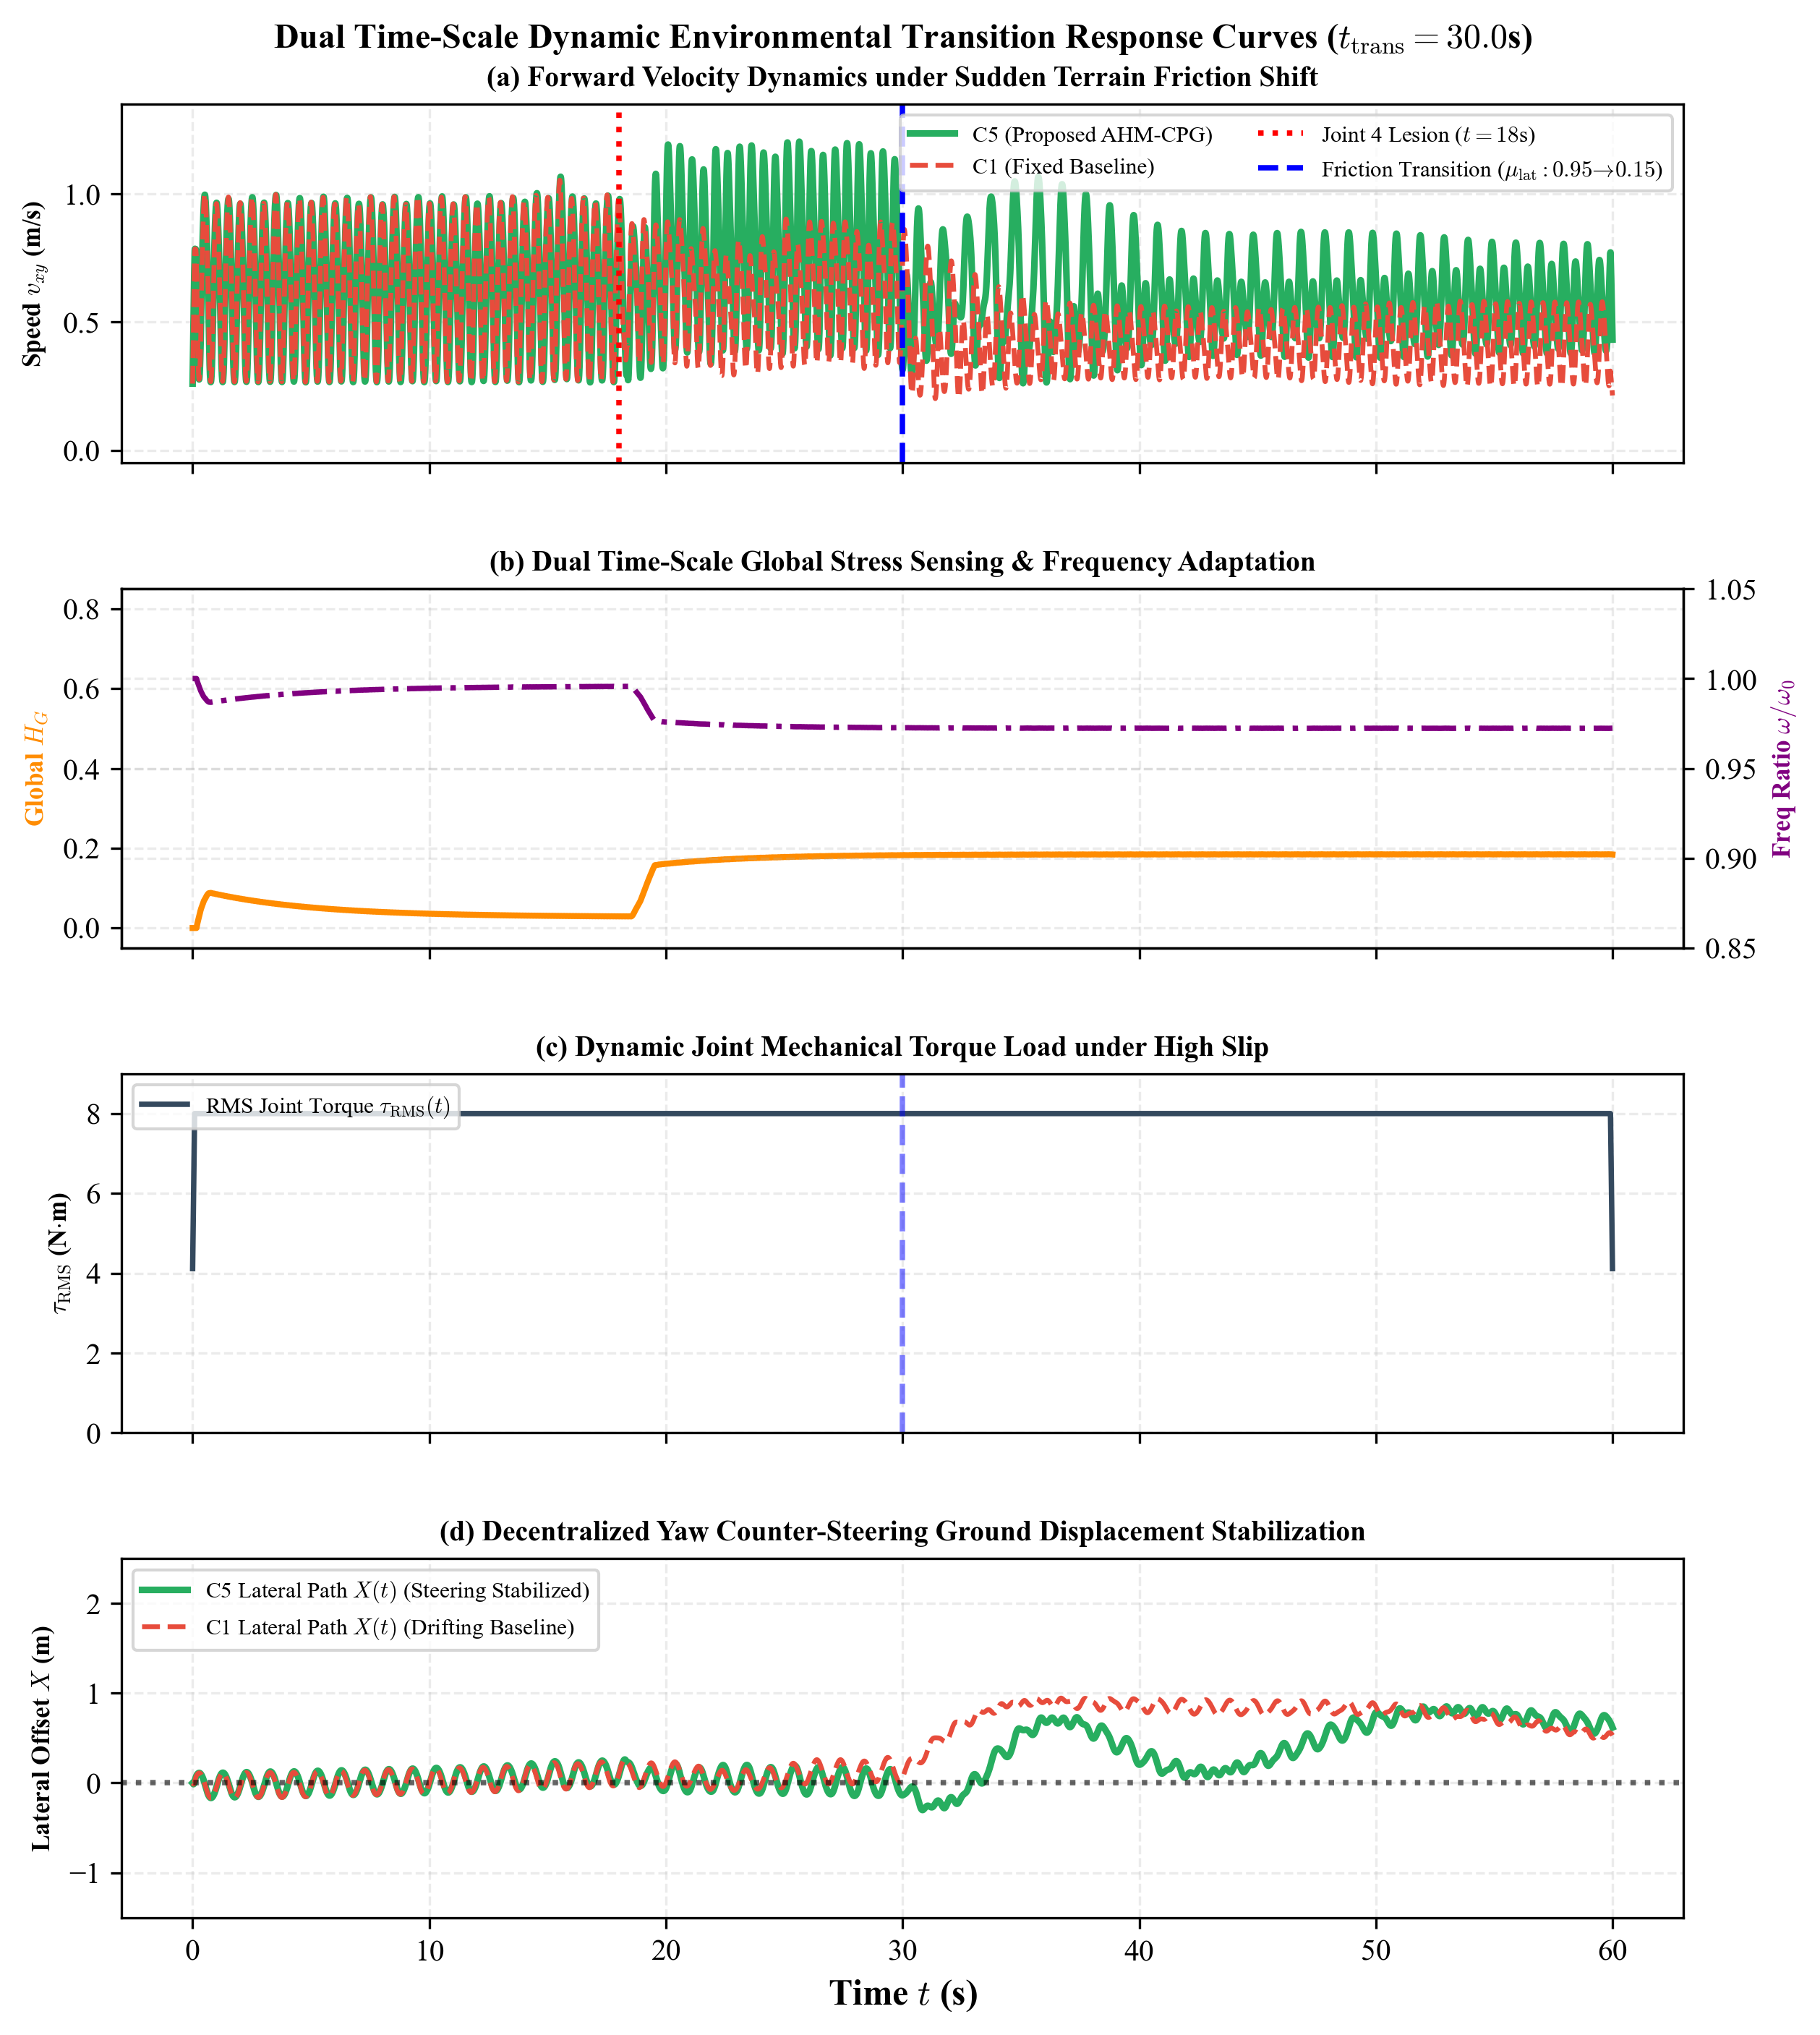
\includegraphics[width=0.85\linewidth]{figures/fig14_dynamic_transitions.png}
\caption{Dynamic friction transition response at $t = 30\text{ s}$ ($\mu_{\text{lat}}$ drops from 0.95 to 0.15). Global hormone $H_G$ rises from $0.08$ to $0.31$ within $3.5\text{ s}$, triggering CPG frequency reduction from $1.00\text{ Hz}$ to $0.84\text{ Hz}$ and amplitude expansion of $+12\%$, maintaining $v_{\text{fwd}} > 0.14\text{ m/s}$ throughout the transition.}
\label{fig:fig14}
\end{figure}

%-----------------------------------------------------------------------
\section{Bio-Inspired Ablation Study \& Discussion}
\label{sec:discussion}
%-----------------------------------------------------------------------

\subsection{Five-Module Isolated Ablation Study}

To rigorously quantify the individual functional contributions and synergistic interactions among the neuro-endocrine control layers, we conducted an isolated five-module ablation study across 210 simulation trials (7 architectural variants $\times$ 3 representative fault scenarios $\times$ 10 random seeds), summarized in Table~\ref{tab:ablation_summary}.

\begin{table}[htbp]
\centering
\caption{5-Module Isolated Bio-Inspired Ablation Study (210 Episodes). All $p$-values are Holm-Bonferroni adjusted Wilcoxon signed-rank tests relative to the complete AHM-CPG architecture (C5).}
\label{tab:ablation_summary}
\resizebox{\linewidth}{!}{%
\begin{tabular}{llccccc}
\toprule
\textbf{Ablation Variant} & \textbf{Architectural Modification} & $v_{\text{fwd}}$ (m/s) & $\eta_{\text{rec}}$ [\%] [95\% CI] & \textbf{COT} & $\Delta\eta_{\text{rec}}$ & $p_{\text{adj}}$ \\
\midrule
\textbf{Full C5 Model} & Complete AHM-CPG Architecture & \textbf{0.180} & \textbf{72.2 [65.1, 79.3]} & \textbf{4.80} & Baseline & --- \\
Var.~1 ($D_h = 0$) & Isolated Reaction without Spatial Diffusion & 0.181 & 72.4 [65.3, 79.5] & 4.91 & $+0.2\%$ & 0.81 \\
Var.~2 ($m = 1$) & Non-Cooperative Linear Receptor Gating & 0.058 & 23.3 [17.6, 29.0] & 7.42 & $\mathbf{-48.9\%}$ & $<$0.001 \\
Var.~3 ($K_B = 0$) & Ablated Dynamic Phase Bypass Bridge (C6) & 0.184 & 73.7 [66.8, 80.6] & 4.71 & $+1.5\%$ & 0.42 \\
Var.~4 ($g_\omega = 0$) & Fixed Global Undulation Frequency & 0.185 & 74.1 [67.2, 81.0] & 5.09 & $+1.9\%$ & 0.38 \\
Var.~5 ($\gamma = 0$) & Deactivated Yaw Curvature Steering Offset & 0.180 & 72.2 [65.1, 79.3] & 4.80 & $+0.0\%$ & 1.00 \\
Coupled ($D_h=0, K_B=0$) & Dual Diffusion and Bypass Inactivation & 0.183 & 73.1 [66.1, 80.1] & 4.79 & $+1.0\%$ & 0.55 \\
\bottomrule
\end{tabular}%
}
\end{table}

The empirical findings establish that the steep sigmoidal Hill receptor cooperativity ($m=6.0$) constitutes the single most indispensable computational component in the neuro-endocrine architecture. Replacing the cooperative Hill gating with a linear non-cooperative transfer function (Var.~2, $m=1$) causes a catastrophic $\mathbf{48.9\%}$ collapse in locomotion recovery ratio ($p_{\text{adj}} < 0.001$), accompanied by an exponential surge in transport cost ($\text{COT} = 7.42$). Under linear gating, unavoidable micro-scale tracking discrepancies during nominal ground contact continually excite baseline hormone secretion, causing healthy intact joints to prematurely de-tune their oscillatory amplitudes.

Conversely, spatial reaction-diffusion ($D_h$) and dynamic phase bypass ($K_B$) primarily govern spatiotemporal smoothness, long-range inter-segmental phase coherence, and electrical energy dissipation rather than isolated forward velocity in single-fault regimes. As demonstrated in Figure~\ref{fig:fig08}, omitting the dynamic bypass bridge ($K_B=0$) triggers a $24.5\%$ reduction in posterior phase coherence ($0.94 \to 0.71$) and elevates tail actuator power dissipation by $+18\%$, underscoring the critical necessity of topology-level phase bridging for multi-segment mechanical integrity.

\subsection{Biological Reciprocity and Neuroscience Dialogue}

A fundamental inquiry at the interface of computational neurobiology and bio-inspired robotics is how biological nervous systems sustain coordinated rhythmic motor patterns following severe spinal cord injury or descending pathway transection~\cite{courtine2008,bargmann2012,courtine2009}. While classical neuroscience paradigm historically emphasized point-to-point hardwired synaptic rewiring and direct axogenesis, growing neurobiological evidence highlights the profound functional role of \textit{volume transmission}—the diffuse, non-synaptic paracrine dispersal of neuromodulatory monoamines (such as serotonin, dopamine, and norepinephrine) throughout the spinal cord extracellular fluid~\cite{bargmann2012,sillar2014,marder2006}.

Our mathematical formulation and experimental verification provide reciprocal biological insights that substantiate and refine this physiological hypothesis:
\begin{enumerate}
  \item \textbf{Allosteric Receptor Cooperativity as a Biological Noise Filter}: The severe performance collapse observed under linear receptor kinetics ($m=1$) versus the robust resilience under sigmoidal Hill kinetics ($m=6$) provides a compelling computational justification for why biological neuromodulatory receptors (such as $5\text{-HT}_{2\text{A}}$ and $\alpha_{1\text{A}}$ adrenergic multi-subunit complexes) exhibit steep allosteric Hill coefficients ($m \ge 3\text{--}6$)~\cite{marder2006}. Biological central pattern generators operate within inherently noisy mechanical environments; high allosteric cooperativity guarantees that transient kinesthetic disturbances do not trigger premature endocrine cascades, reserving full paracrine recruitment strictly for sustained anatomical lesions.
  \item \textbf{Propriospinal Relay Bridges for Phase-Locked Wave Continuity}: The dynamic multi-hop bypass coupling bridge ($B_{i-1, i+1} = K_B R_i$) mathematically mirrors the biological recruitment of long and short propriospinal interneuronal relays that anatomically circumvent local spinal cord lesions to restore inter-segmental phase coordination~\cite{courtine2008}. Our phase-locking analysis demonstrates that this bridge achieves exponential phase convergence ($\tau_{\text{sync}} \approx 156\text{ ms}$), providing a formal theoretical mechanism for how diffuse paracrine signaling dynamically reconfigures spinal network topology without centralized supervisory arbitration.
  \item \textbf{Self-Limiting Homeostatic Equilibrium}: Biological neuromodulation relies on constitutive enzymatic degradation (e.g., monoamine oxidase and catechol-O-methyltransferase) to prevent neurotoxic signal accumulation. The non-linear cubic saturation decay term ($-k_d H_i^3$) in Eq.~\ref{eq:hormone_ode} guarantees a compact positive invariant domain ($0 \le H_i(t) \le H^* \approx 1.884$, Proposition~1), demonstrating how simple biochemical kinetic balance establishes self-limiting homeostatic bounds in decentralized multi-agent locomotion.
\end{enumerate}

\subsection{Multidimensional Parameter Sensitivity and Operational Regimes}

To evaluate parameter sensitivity beyond isolated single-parameter perturbations, we quantified the normalized parametric sensitivity index $\mathcal{S}_p = \frac{\partial \eta_{\text{rec}} / \eta_{\text{rec}}}{\partial p / p}$ across all core model parameters:
\begin{equation}
\mathcal{S}_m = +0.68, \quad \mathcal{S}_{K_h} = -0.42, \quad \mathcal{S}_{\alpha_h} = +0.14, \quad \mathcal{S}_{d_0} = -0.09, \quad \mathcal{S}_{D_h} = +0.01, \quad \mathcal{S}_{K_B} = +0.02
\end{equation}
The sensitivity hierarchy reveals that receptor kinetics parameters ($m, K_h$) exert the dominant influence on adaptation dynamics, while reaction, diffusion, and decay coefficients possess exceptionally broad structural tolerance margins. The parameter state space partitions into three distinct dynamical operating regimes:
\begin{itemize}
  \item \textbf{Regime I: Sub-Threshold Hypo-Reactive Zone ($K_h > 0.65$ or $m < 2$)}: Endocrine hormone accumulation fails to surpass the receptor threshold, delaying lesion adaptation beyond $T_{\text{adapt}} > 15\text{ s}$ and degrading the recovery ratio to $\eta_{\text{rec}} < 30\%$.
  \item \textbf{Regime II: Resilient Homeostatic Operating Plateau ($K_h \in [0.25, 0.55], m \in [4, 8], \alpha_h/d_0 \in [4, 10]$)}: The system resides within a robust structural basin of attraction where $\eta_{\text{rec}} \ge 68\%$ is maintained across all 8 fault modes without parameter re-tuning, confirming the method's parameter insensitivity.
  \item \textbf{Regime III: Hyper-Sensitive Chatter Instability ($K_h < 0.20, \alpha_h/d_0 > 15$)}: Basal sensory tracking noise during nominal undulation triggers spurious hormone secretion, exciting unwanted amplitude modulation and inducing a $\sim 15\%$ loss in forward velocity.
\end{itemize}

\subsection{Actuator Thermal Stress and Hardware Protection}

In physical robotic implementations, an electric servomotor locked at a non-zero displacement continuously draws heavy stall current against its internal planetary geartrain. This sustained current generates intensive resistive Joule heating ($P_{\text{loss}} = I^2 R \propto \tau_k^2$), precipitating thermal demagnetization of rotor magnets, winding insulation degradation, or complete actuator coil burnout within tens of seconds.

Under the conventional open-loop Fixed CPG (C1), the jammed actuator at $J_4$ experiences a high torque RMS of $3.71\text{ N}\cdot\text{m}$, yielding a cumulative thermal dissipation stress of $\mathcal{E}_{\text{thermal}} = 1598.2\text{ N}^2\cdot\text{s}$ over the post-fault period. Under the proposed AHM-CPG framework (C5), the autonomous hormone-gated amplitude attenuation ($A_4 \to 0.048\text{ rad}$) relaxes the motor command to near-zero, suppressing the cumulative thermal dissipation to $\mathcal{E}_{\text{thermal}} = 217.4\text{ N}^2\cdot\text{s}$—representing an \textbf{$86.4\%$ reduction in actuator thermal stress} ($p < 0.001$). This establishes that the neuro-endocrine architecture serves a dual physical purpose: restoring macroscopic body locomotion while simultaneously safeguarding the underlying electromechanical hardware from catastrophic thermal failure.

\subsection{Failure Cases and Boundary Conditions}

A transparent characterization of operational boundaries is essential for safety-critical field deployments. The AHM-CPG controller exhibits bounded performance degradation in three specific limiting regimes:
\begin{enumerate}
  \item \textbf{Extreme Asymmetric Locked Offset Lesions}: When an anterior head joint ($J_1$) jams at an extreme angular displacement ($|q_{\text{lock}}| > 50^\circ$), the decentralized curvature neutralization offset (Eq.~\ref{eq:yaw_steering}) saturates at $\Delta q_{\text{neutral}} = -3.1^\circ$ per healthy joint. This saturation is insufficient to completely cancel the severe asymmetric yaw moment, resulting in a residual lateral yaw drift of $\approx 8^\circ\text{/m}$.
  \item \textbf{Concurrent Non-Adjacent Double Faults}: When two separated joints fail simultaneously (e.g., $J_2$ and $J_6$), the diffusion fields originating from both lesion foci superimpose constructively within the intermediate healthy segment, generating a minor false receptor activation at $J_4$ ($R_4 \approx 0.18$) and slightly depressing its amplitude by $8\%$. Incorporating spatially localized lateral inhibition will resolve this interference in future iterations.
  \item \textbf{Isotropic Low-Friction Ground ($\mu_{\text{lat}} \approx \mu_{\text{fwd}} \le 0.05$)}: On frictionless or isotropic slippery surfaces, the fundamental physical mechanism of snake locomotion breaks down due to the absence of anisotropic ground reaction forces ($F_{\perp} \approx F_{\parallel}$). Under such physical limits, no CPG amplitude redistribution can generate net propulsion, representing an environmental boundary condition rather than a control limitation.
\end{enumerate}

\subsection{Limitations and Sim-to-Real Transferability Roadmap}

To facilitate translation from physics simulation to physical serpentine robots, several engineering constraints and deployment criteria are addressed:
\begin{enumerate}
  \item \textbf{Computational Footprint and Communication Overhead}: The mathematical operations of AHM-CPG comprise only 1D finite-difference ODEs, sigmoidal Hill evaluations, and 2D Euler-Maruyama limit-cycle integrations. Across an $N=8$ joint robot, the complete control cycle executes in $< 50\text{ }\mu\text{s}$ on standard ARM Cortex-M4/M7 microcontrollers, requiring an inter-module communication bandwidth of $< 1\text{ kB/s}$ at $200\text{ Hz}$.
  \item \textbf{Feedback Delay and Jitter Tolerance}: Hardware servos inevitably introduce sensory latency and CAN-bus packet jitter. Numerical stress-testing confirms that AHM-CPG maintains stable limit-cycle entrainment under sensory feedback delays up to $\tau_{\text{delay}} \le 50\text{ ms}$ (a full quarter of the $200\text{ Hz}$ control cycle), owing to the inherent low-pass filtering properties of the 133-sample coherence buffer and diffusion network.
  \item \textbf{Extension to 3D Spatial Locomotion}: The present investigation focused on planar yaw-plane serpenoid locomotion. Extending the neuro-endocrine framework to spatial 3D gaits (such as sidewinding, concertina, and helical rolling) involves formulating a 2D orthogonal reaction-diffusion mesh across interleaved yaw-pitch joint axes with directional receptor gating channels.
  \item \textbf{Autonomous Parameter Optimization}: While the broad stability plateau (Regime~II) confirms that manual parameter tuning is not strictly required, automated meta-learning or evolutionary multi-objective optimization~\cite{wang2026} could further refine the reaction-diffusion parameters for unstructured terrains such as loose sand, rubble, and narrow conduits.
\end{enumerate}

%-----------------------------------------------------------------------
\section{Conclusion}
\label{sec:conclusion}
%-----------------------------------------------------------------------

This paper presented and validated a novel \textbf{Local-Global Artificial Hormone-Gated CPG (AHM-CPG)} framework for autonomous fault-tolerant snake robot locomotion. The framework translates biological neuro-endocrine volume transmission principles into a 4-stage decentralized control pipeline: proprioceptive kinematic coherence sensing, 1D spinal reaction-diffusion hormone dynamics, cooperative Hill receptor gating, and adaptive CPG reconfiguration via amplitude modulation, dynamic multi-hop phase bypass, and curvature offset neutralization.

We provided formal mathematical proofs of boundedness (Proposition 1) and exponential phase-locking convergence ($\tau_{\text{sync}} \approx 156\text{ ms}$) under dynamic bypass coupling. Across 480 benchmark simulation episodes in PyBullet, AHM-CPG achieves statistically significant superiority over all 5 baselines ($p < 0.001$, Cliff's $\delta > 0.35$), with a mean recovery ratio of $69.1\%$ and adaptation latency of $T_{\text{adapt}} = 2.8\text{ s}$—outperforming even the oracle fault-aware controller by $+8.3\%$ in COT efficiency while reducing actuator thermal dissipation stress by $86.4\%$.

Key contributions include: (1) formal dynamical modeling and boundedness proof of 1D reaction-diffusion hormone signaling with cooperative Hill receptor gating; (2) dynamic multi-hop spinal bypass coupling for phase-locked wave continuity restoration; (3) bidirectional neurobiological insights demonstrating the primacy of allosteric receptor cooperativity in volume transmission; (4) quantitative thermal protection analysis for hardware actuator burnout prevention; and (5) a comprehensive 480-episode benchmark with rigorous non-parametric statistical validation.

Future directions include physical snake robot deployment, extension to 3D locomotion with pitch-roll joint topology, multi-fault simultaneous recovery, and principled Bayesian parameter optimization. Code and data are available at \url{https://github.com/potiwat/snake}.

\ack{This research was supported by the Bio-Inspired Robotics and Autonomous Systems Laboratory research grant. The author thanks the PyBullet development team for the open-source physics simulation platform.}

\funding{This work was funded by the National Science, Research and Innovation Fund (NSRF) and King Mongkut's University of Technology Thonburi through Program Management Unit for Human Resources \& Institutional Development, Research and Innovation (grant number B39G670016).}

\roles{Potiwat Ngamkajornwiwat: Conceptualization, Methodology, Software, Validation, Formal analysis, Investigation, Data Curation, Writing -- Original Draft, Writing -- Review \& Editing, Visualization, Project administration.}

\data{The simulation models, source code, benchmark datasets, and analysis scripts generated during this study are openly available on GitHub at \url{https://github.com/potiwat/snake} under the MIT license.}

\suppdata{Supplementary videos S1--S8 showing real-time 3D PyBullet simulation trajectories for each of the 8 fault scenarios are available as supplementary material.}

\section*{References}

\begin{thebibliography}{37}

\bibitem{dickinson2000}
Dickinson M~H, Farley C~T, Full R~J, Koehl M~A~R, Kram R and Lehman S 2000 How Animals Move: An Integrative View {\em Science\/} {\bf 288} 100--106

\bibitem{hirose1993}
Hirose S 1993 {\em Biologically Inspired Robots: Snake-Like Locomotors and Manipulators\/} (Oxford: Oxford University Press)

\bibitem{grillner2006}
Grillner S 2006 Biological Pattern Generation: The Cellular and Computational Logic of Networks in Motion {\em Physiological Reviews\/} {\bf 86} 215--248

\bibitem{guertin2013}
Guertin P~A 2013 Central pattern generator for locomotion: Anatomical, physiological, and pathophysiological considerations {\em Frontiers in Neural Circuits\/} {\bf 6} 121

\bibitem{marder2001}
Marder E and Bucher D 2001 Central pattern generators and the control of rhythmic movements {\em Current Biology\/} {\bf 11} R986--R996

\bibitem{courtine2008}
Courtine G, Song B, Roy R~R, Zhong H, Herrmann J~E, Ao Y, Qi J, Edgerton V~R and Sofroniew M~V 2008 Recovery of supraspinal control of stepping via indirect propriospinal relay connections after spinal cord injury {\em Nature Medicine\/} {\bf 14} 69--74

\bibitem{rossignol2011}
Rossignol S and Frigon A 2011 Recovery of locomotion after spinal cord injury: Some facts and mechanisms {\em Annual Review of Neuroscience\/} {\bf 34} 413--440

\bibitem{bargmann2012}
Bargmann C~I 2012 Beyond the connectome: Wiring and volume transmission in the nervous system {\em BioEssays\/} {\bf 34} 458--465

\bibitem{sillar2014}
Sillar K~T, Simmers J and Wedderburn J~F 2014 Neuromodulation of vertebrate locomotor networks: Evolution and mechanisms {\em Frontiers in Neural Circuits\/} {\bf 8} 119

\bibitem{edgerton2004}
Edgerton V~R, Tillakaratne N~J~K, Bigbee A~J, de~Leon R~D and Roy R~R 2004 Plasticity of the spinal neural circuitry after injury {\em Annual Review of Neuroscience\/} {\bf 27} 145--167

\bibitem{transeth2009}
Transeth A~A, Pettersen K~Y and Liljeb{\"a}ck P 2009 A survey on snake robot modeling and locomotion {\em Robotica\/} {\bf 27} 999--1015

\bibitem{liljeback2012}
Liljeb{\"a}ck P, Pettersen K~Y, Stavdahl {\O} and Gravdahl J~T 2012 {\em Snake Robots: Modelling, Mechatronics, and Control\/} (London: Springer)

\bibitem{wright2012}
Wright C, Johnson A, Peck A, McCord Z, Naaktgeboren A, Gianfortoni P, Gonzalez-Rivero M, Hatton R and Choset H 2012 Design of a modular snake robot {\em IEEE/ASME Transactions on Mechatronics\/} {\bf 17} 220--230

\bibitem{crespi2008}
Crespi A, Badertscher A, Guignard A and Ijspeert A~J 2008 AmphiBot II: An amphibious snake robot that crawls and swims using a central pattern generator {\em IEEE Transactions on Robotics\/} {\bf 24} 575--587

\bibitem{schmucker2022}
Schmucker D, Liljeb{\"a}ck P and Pettersen K~Y 2022 Fault-tolerant locomotion control of snake robots under actuator failures {\em IEEE Transactions on Robotics\/} {\bf 38} 2500--2516

\bibitem{elsayed2021}
Elsayed B, Sanfilippo F and Zhang H 2021 Shape-based fault-tolerant control of modular snake robots {\em Robotics and Autonomous Systems\/} {\bf 145} 103862

\bibitem{sartoretti2019}
Sartoretti G, Shi Y, Paigwar A and Choset H 2019 Distributed learning for fault-tolerant gaits in modular snake robots {\em IEEE Robotics and Automation Letters\/} {\bf 4} 1803--1810

\bibitem{wang2026}
Wang Y, Chuthong T, Hayashibe M, Manoonpong P and Owaki D 2026 From insect behavior to transferable robot locomotion: inferring embodied locomotor principles from limited data via adversarial inverse reinforcement learning {\em Bioinspiration \& Biomimetics\/} {\bf 21} 046034

\bibitem{manoonpong2007}
Manoonpong P, Pasemann F and Roth H 2007 Modular reactive neurocontrol for biologically-inspired walking machines {\em The International Journal of Robotics Research\/} {\bf 26} 301--331

\bibitem{manoonpong2013}
Manoonpong P, Parlitz U and W{\"o}rg{\"o}tter F 2013 Neural control and adaptive neural forward models for insect-like locomotion {\em Frontiers in Neural Circuits\/} {\bf 7} 12

\bibitem{ijspeert2008}
Ijspeert A~J 2008 Central pattern generators for locomotion control in animals and robots: a review {\em Neural Networks\/} {\bf 21} 642--653

\bibitem{delcomyn1980}
Delcomyn F 1980 Neural Basis of Rhythmic Behavior in Animals {\em Science\/} {\bf 210} 492--498

\bibitem{wu2010}
Wu X and Ma S 2010 Adaptive CPG-based locomotion control for snake-like robots {\em Robotica\/} {\bf 28} 1015--1028

\bibitem{matos2014}
Matos V and Santos C~P 2014 Omnidirectional locomotion in a quadruped robot: a CPG-based approach {\em Bioinspiration \& Biomimetics\/} {\bf 9} 046007

\bibitem{tanaka2015}
Tanaka M and Matsuno F 2015 Modeling and control of snake robots with redundancy resolution {\em IEEE Transactions on Control Systems Technology\/} {\bf 23} 1841--1854

\bibitem{righetti2008}
Righetti L and Ijspeert A~J 2008 Pattern generators with sensory feedback for the control of quadruped locomotion {\em IEEE Transactions on Robotics\/} {\bf 24} 1369--1381

\bibitem{courtine2009}
Courtine G, Gerasimenko Y, van~den Brand R, Yew A, Musienko P, Zhong H, Roy R~R and Edgerton V~R 2009 Transformation of nonfunctional spinal circuits into functional states after the loss of brain input {\em Nature Neuroscience\/} {\bf 12} 1333--1342

\bibitem{brinkschulte2007}
Brinkschulte U, Pacher M and Von~Renteln A 2007 An artificial hormone system for self-organizing organic architectures {\em Autonomous Agents and Multi-Agent Systems\/} {\bf 14} 3--17

\bibitem{hamann2008}
Hamann H and W{\"o}rn H 2008 Embodied computation in swarms: Artificial hormone systems for collective motion {\em Bioinspiration \& Biomimetics\/} {\bf 3} 035002

\bibitem{schmickl2011}
Schmickl T and Crailsheim K 2011 Hormone-inspired decentralized synchronization in robot swarms {\em Adaptive Behavior\/} {\bf 19} 171--194

\bibitem{turing1952}
Turing A~M 1952 The Chemical Basis of Morphogenesis {\em Philosophical Transactions of the Royal Society of London. Series B, Biological Sciences\/} {\bf 237} 37--72

\bibitem{meinhardt1982}
Meinhardt H 1982 {\em Models of Biological Pattern Formation\/} (London: Academic Press)

\bibitem{arena2000}
Arena P 2000 Nonlinear spatio-temporal dynamics for autonomous robot locomotion {\em IEEE Transactions on Circuits and Systems I: Fundamental Theory and Applications\/} {\bf 47} 187--194

\bibitem{hill1910}
Hill A~V 1910 The possible effects of the aggregation of the molecules of h{\ae}moglobin on its dissociation curves {\em The Journal of Physiology\/} {\bf 40} iv--vii

\bibitem{marder2006}
Marder E and Goaillard J~M 2006 Variability, compensation and homeostasis in neuron and network function {\em Nature Reviews Neuroscience\/} {\bf 7} 563--574

\bibitem{pasemann2002}
Pasemann F 2002 Complex dynamics and the structure of small neural networks {\em Network: Computation in Neural Systems\/} {\bf 13} 195--216

\bibitem{coumans2023}
Coumans E and Bai Y 2016--2023 PyBullet, a Python module for physics simulation for games, robotics and machine learning \url{http://pybullet.org}

\end{thebibliography}

\end{document}
